\subsection{Mackey topology and weakened topology on a locally convex space}

Let E be a locally convex space and \(E'\) its dual. We put E and \(E'\) in duality by means of the canonical bilinear form \((x, x') \mapsto \langle x, x' \rangle\) on \(E \times E'\) . This duality is separating in \(E'\) . We shall consider three topologies on E compatible with the duality between E and \(E'\) :

\begin{enumerate}
\def\labelenumi{\alph{enumi})}
\item
  the given topology on E, which we shall call the initial topology, whenever any confusion is likely to arise;
\item
  the topology \(\sigma(\mathrm{E},\mathrm{E}^{\prime})\) , called the weakened topology on \(\mathrm{E}\) ;
\item
  the topology \(\tau(\mathrm{E},\mathrm{E}')\) , called the Mackey topology on E.
\end{enumerate}

The initial topology is finer than the weakened topology and coarser than the Mackey topology; moreover, these three topologies can be distinct (IV, p.~49, exerc. 8).

By prop. 1 of IV, p.~1, these three topologies have the same closed convex sets, the same barrels, the same bounded sets and the same adapted bornologies. In particular :

PROPOSITION 2. --- Let E be a locally convex space, and let A be a convex subset of E (for example, a vector subspace of E). The closure of A is the same for the initial topology and for the weakened topology of E.

Remarks. --- 1) For a family \((x_{i})_{i\in\mathbf{I}}\) of elements of E to be total (resp. topologically independent) for the initial topology, it is necessary and sufficient that it is so for the weakened topology; this follows from prop. 2. Hence we can apply the criteria of II, p.~43.

\begin{enumerate}
\def\labelenumi{\arabic{enumi})}
\setcounter{enumi}{1}
\tightlist
\item
  Let \(\mathcal{T}_1\) and \(\mathcal{T}_2\) be two locally convex topologies on E, compatible with the duality between E and E', \(\mathcal{T}_1\) being finer than \(\mathcal{T}_2\) . Then every neighbourhood of 0 for \(\mathcal{T}_1\) , which is convex and closed for \(\mathcal{T}_1\) is closed for \(\mathcal{T}_2\) by prop. 1 of IV, p.~1. Consequently (GT, II, § 3, No.~3, corollary) every subset of E which is complete for \(\mathcal{T}_2\) is so for \(\mathcal{T}_1\) also.
\end{enumerate}

In particular, every subset of E which is complete for the weakened topology is complete for the initial topology, and every subset of E complete for the initial topology is so for the Mackey topology. If E is quasi-complete for the weakened topology, it is so for every topology compatible with the duality between E and E'. If it is quasi-complete for the initial topology, it is so for the Mackey topology.

\begin{enumerate}
\def\labelenumi{\arabic{enumi})}
\setcounter{enumi}{2}
\tightlist
\item
  Suppose E is Hausdorff (for the initial topology). Let A be a subset of E which is closed and bounded for \(\sigma(\mathrm{E}, \mathrm{E}')\) , hence also for every topology compatible with the duality between E and \(E'\) . Since A is precompact for \(\sigma(\mathrm{E}, \mathrm{E}')\) (III, p.~3, Remark 5), assuming that A is compact for \(\sigma(\mathrm{E}, \mathrm{E}')\) is equivalent to A being complete for \(\sigma(\mathrm{E}, \mathrm{E}')\) .
\end{enumerate}

Therefore, on account of remark 2, we see that :

PROPOSITION 3. --- Suppose E is Hausdorff, and E' its dual. Every subset of E which is precompact for the initial topology and compact for \(\sigma(E, E')\) , is compact for the initial topology.

\begin{enumerate}
\def\labelenumi{\arabic{enumi})}
\setcounter{enumi}{3}
\tightlist
\item
  The topology \(\beta(\mathrm{E},\mathrm{E}')\) (IV, p.~4, def. 3) is finer than the Mackey topology. If \(\beta(\mathrm{E},\mathrm{E}')\) is distinct from \(\tau(\mathrm{E},\mathrm{E}')\) , it is not compatible with the duality between E and E'. The space E is barrelled if and only if the initial topology is equal to \(\beta(\mathrm{E},\mathrm{E}')\) (III, p.~24).
\end{enumerate}

PROPOSITION 4. --- Let E be a locally convex space. The Mackey topology on E is identical with the initial topology in each of the following cases :

\begin{enumerate}
\def\labelenumi{\alph{enumi})}
\item
  E is barrelled;
\item
  E is bornological;
\item
  E is metrizable.
\end{enumerate}

We note first that the Mackey topology on E is identical with the initial topology if and only if every convex subset of \(E'\) which is compact for \(\sigma(E', E)\) , is equi-continuous. This is certainly the case if E is barrelled (III, p.~24, corollary).

Suppose E is bornological; let V be a convex and balanced neighbourhood of 0 in E for the topology \(\tau(E, E')\) . Let B be a subset of E, bounded for the initial topology. Since B is bounded for the Mackey topology, V absorbs B, and since E is bornological, V is a neighbourhood of 0 for the initial topology.

In case c), the space E is bornological (III, p.~12, prop. 2).

\subsection{Transpose of a continuous linear mapping}

In this section, \(E_{1}\) and \(E_{2}\) denote two locally convex spaces, with respective duals \(E_{1}^{\prime}\) and \(E_{2}^{\prime}\) .

Let \(u\) be a linear mapping from \(\mathrm{E}_1\) into \(\mathrm{E}_2\) . For \(u\) to be continuous when \(\mathrm{E}_1\) and \(\mathrm{E}_2\) are assigned the weakened topologies, it is necessary and sufficient that \(f \circ u\) belongs to \(\mathrm{E}_1'\) for all \(f \in \mathrm{E}_2'\) ; this is the case if \(u\) is continuous. Then the linear mapping \(f \mapsto f \circ u\) from \(\mathrm{E}_2'\) into \(\mathrm{E}_1'\) is called the transpose of \(u\) and is denoted by \(^t u\) .

PROPOSITION 5. --- Let u be a continuous linear mapping from \(E_{1}\) into \(E_{2}\) .

\begin{enumerate}
\def\labelenumi{(\roman{enumi})}
\item
  If \(E_{1}\) and \(E_{2}\) are Hausdorff then u is injective if and only if the image of \(^{t}u\) is dense in \(E_{1}^{\prime}\) for the weak topology \(\sigma(\mathrm{E}_{1}^{\prime},\mathrm{E}_{1})\) .
\item
  For \({}^{t}u\) to be injective it is necessary and sufficient that the image of \(u\) is dense in \(\mathbf{E}_2\) .
\end{enumerate}

A vector subspace of \(E_{2}\) is dense for the initial topology if and only if it is dense for the weakened topology (IV, p.~4, prop. 2). Prop. 5 then follows from II, p.~47, cor. 2.

PROPOSITION 6. --- Let u be a linear mapping from \(E_{1}\) into \(E_{2}\) which is continuous for the weakened topologies. For i = 1, 2, let \(S_{i}\) be a family of bounded subsets of \(E_{i}\) . In order that \(^{t}u\) is a continuous mapping from \((\mathrm{E}_{2}^{\prime})_{\mathfrak{S}_{2}}\) into \((\mathrm{E}_{1}^{\prime})_{\mathfrak{S}_{1}}\) , it is necessary and sufficient that, for every set \(A \in S_{1}\) , there exist sets \(A_{1}, \ldots, A_{n}\) in \(S_{2}\) and a real number \(\lambda > 0\) such that \(\lambda.u(\mathbf{A})\) is contained in the closed convex balanced envelope of \(A_{1} \cup \ldots \cup A_{n}\) .

This is an immediate consequence of prop. 2 of III, p.~15.

COROLLARY. --- Let u be a continuous linear mapping from \(E_{1}\) into \(E_{2}\) . Then \({}^t u\) is continuous when the duals \(E_{i}'\) are assigned the following topologies :

\begin{enumerate}
\def\labelenumi{\alph{enumi})}
\item
  the weak topologies \(\sigma (\mathrm{E}_i^{\prime},\mathrm{E}_i)\)
\item
  the strong topologies \(\beta (\mathrm{E}_i^{\prime},\mathrm{E}_i)\)
\item
  the Mackey topologies \(\tau (\mathrm{E}_i^{\prime},\mathrm{E}_i)\)
\item
  the topologies of precompact convergence.
\end{enumerate}

Moreover, if \(E_{2}\) is Hausdorff, \(^{t}u\) is continuous when the duals \(E_{i}^{\prime}\) are assigned:

\begin{enumerate}
\def\labelenumi{\alph{enumi})}
\setcounter{enumi}{4}
\tightlist
\item
  the topologies of compact convergence (resp. compact convex).
\end{enumerate}

The only point which requires a proof is the case \(c\) ), when the topologies of \(\mathrm{E}_1\) and \(\mathrm{E}_2\) are not necessarily Hausdorff. Then for every linear form \(f \in \mathrm{E}'_1{}^*\) , \(f \circ {}^t u\) is a linear form on \(\mathrm{E}_2'\) ; hence there is a linear mapping \(v: \mathrm{E}'_1{}^* \to \mathrm{E}'_2{}^*\) which is continuous for the topologies \(\sigma(\mathrm{E}'_1{}^*, \mathrm{E}'_1)\) and \(\sigma(\mathrm{E}'_2{}^*, \mathrm{E}'_2)\) and is such that \(d_{\mathrm{B}_2} \circ u = v \circ d_{\mathrm{B}_1}\) , where \(d_{\mathrm{B}_i}\) is the canonical mapping from \(\mathrm{E}_i\) into \(\mathrm{E}'_i{}^* (i = 1, 2)\) . Consequently, if A is a subset of \(\mathrm{E}_1\) such that \(d_{\mathrm{B}_1}(\mathrm{A})\) is convex, balanced and compact for \(\sigma(\mathrm{E}'_1{}^*, \mathrm{E}'_1)\) then \(d_{\mathrm{B}_2}(u(\mathrm{A})) = v(d_{\mathrm{B}_1}(\mathrm{A}))\) is convex, balanced and compact for \(\sigma(\mathrm{E}'_2{}^*, \mathrm{E}'_2)\) since the topologies \(\sigma(\mathrm{E}'_1{}^*, \mathrm{E}'_1)\) and \(\sigma(\mathrm{E}'_2{}^*, \mathrm{E}'_2)\) are Hausdorff.

PROPOSITION 7. --- Let \(u: \mathrm{E}_1 \to \mathrm{E}_2\) be a linear mapping. We assume that \(u\) is continuous for the weakened topologies of \(\mathrm{E}_1\) and \(\mathrm{E}_2\) .

\begin{enumerate}
\def\labelenumi{(\roman{enumi})}
\item
  The mapping \(u\) is continuous if \(\mathrm{E}_1\) and \(\mathrm{E}_2\) are assigned their Mackey topologies.
\item
  If \(\mathbf{E}_1\) is bornological or barrelled, then \(u\) is continuous for the initial topologies of \(\mathbf{E}_1\) and \(\mathbf{E}_2\) .
\item
  In order that \(u\) be continuous for the initial topologies of \(\mathbf{E}_1\) and \(\mathbf{E}_2\) , it is necessary and sufficient that the image under \(^t u\) of every equicontinuous subset of \(\mathbf{E}_2'\) be equicontinuous in \(\mathbf{E}_1'\) .
\end{enumerate}

The hypothesis implies that \({}^t u\) is continuous for the weak topologies \(\sigma(\mathrm{E}_2', \mathrm{E}_2)\) and \(\sigma(\mathrm{E}_1', \mathrm{E}_1)\) (II, p.~46, corollary) hence the image under \({}^t u\) of a convex, balanced and compact subset for \(\sigma(\mathrm{E}_2', \mathrm{E}_2)\) is convex, balanced and compact for \(\sigma(\mathrm{E}_1', \mathrm{E}_1)\) , the topologies \(\sigma(\mathrm{E}_2', \mathrm{E}_2)\) and \(\sigma(\mathrm{E}_1', \mathrm{E}_1)\) being Hausdorff. Therefore, assertion (i) follows from GT, X, § 1, No.~4, prop. 3, b). Assertion (ii) is a consequence of (i): for, if \(\mathrm{E}_1\) is bornological or barrelled, its initial topology is the Mackey topology, and the Mackey topology of \(\mathrm{E}_2\) is finer than the initial topology of \(\mathrm{E}_2\) . Finally, the initial topology of \(\mathrm{E}_i\) is that of uniform convergence on equicontinuous subsets of \(\mathrm{E}_i'\) (III, p.~19, cor. 1 of prop. 7). This proves (iii).

COROLLARY. --- Suppose \(E_{1}\) is a normed space. Let u be a linear mapping from \(E_{1}\) into \(E_{2}\) . The following properties are equivalent :

\begin{enumerate}
\def\labelenumi{\alph{enumi})}
\item
  \(u\) is continuous;
\item
  \(u\) is continuous for the weakened topologies;
\item
  the image of the unit ball in \(\mathrm{E}_1\) under \(u\) is bounded in \(\mathrm{E}_2\) ;
\item
  for every sequence \((x_{n})\) of points of \(\mathbf{E}_1\) tending to 0 for the initial topology, the sequence \((u(x_{n}))\) is bounded for the weakened topology of \(\mathbf{E}_2\) .
\end{enumerate}

Since \(E_{1}\) is bornological the equivalence of a) and b) follows from prop. 7; that of a) and c) is immediate. The equivalence of a) and d) follows from prop. 1 of IV, p.~1, and from prop. 1 of III, p.~11.

PROPOSITION 8. --- (i) Let E be a normed space, with dual E'. For every \(x \in E\) , we have

\[
\| x \| = \sup _ {x ^ {\prime} \in \mathrm{E} ^ {\prime}, \| x ^ {\prime} \| \leqslant 1} | \langle x, x ^ {\prime} \rangle |.\tag{3}
\]

\begin{enumerate}
\def\labelenumi{(\roman{enumi})}
\setcounter{enumi}{1}
\tightlist
\item
  Let \(\mathbf{E}_1\) and \(\mathbf{E}_2\) be two normed spaces and \(u\) a continuous linear mapping from \(\mathbf{E}_1\) into \(\mathbf{E}_2\) . We have
\end{enumerate}

\[
\left\| ^ {t} u \right\| = \left\| u \right\|.\tag{4}
\]

Let \(x \in E\) . For every \(x' \in E'\) such that \(\| x' \| \leqslant 1\) , we have

\[
\left| \langle x, x ^ {\prime} \rangle \right| \leqslant \| x \| \| x ^ {\prime} \| \leqslant \| x \|.
\]

By Hahn-Banach theorem (II, p.~23, cor. 2), there exists an element \(x'\) in \(E'\) such that \(\| x' \| \leqslant 1\) and \(\langle x, x' \rangle = \| x \|\) . This proves (i).

Let us now prove (ii). By formula (3) and the definition of the transpose, we have

\[
\begin{array}{l} \| ^ {t} u \| = \sup _ {\| y ^ {\prime} \| \leqslant 1} \left\| ^ {t} u (y ^ {\prime}) \right\| = \sup _ {\| y ^ {\prime} \| \leqslant 1, \| x \| \leqslant 1} \left| \langle x, ^ {t} u (y ^ {\prime}) \rangle \right| \\ = \sup _ {\| x \| \leqslant 1, \| y ^ {\prime} \| \leqslant 1} \left| \langle u (x), y ^ {\prime} \rangle \right| = \sup _ {\| x \| \leqslant 1} \left\| u (x) \right\| = \| u \|. \end{array}
\]

Remarks. --- 1) Formula (3) is a particular case of (4), corresponding to the linear mapping \(\lambda \mapsto \lambda x\) from K into E.

\begin{enumerate}
\def\labelenumi{\arabic{enumi})}
\setcounter{enumi}{1}
\tightlist
\item
  Put \(\mathrm{B}(x, y') = \langle u(x), y' \rangle = \langle x, {}^t u(y') \rangle\) for \(x \in \mathrm{E}_1\) , \(y' \in \mathrm{E}_2'\) . The above proof shows that \(\mathbf{B}\) is a continuous bilinear form on \(\mathrm{E}_1 \times \mathrm{E}_2'\) , with norm (GT, X, § 3, No.~2) equal to \(\| u \|\) .
\end{enumerate}

COROLLARY. --- Let E be a normed space satisfying the first axiom of countability. There exists a countable subset D of \(E' - \{0\}\) such that we have

\[
\| x \| = \sup _ {\xi \in \mathbf {D}} | \langle x, \xi \rangle | / \| \xi \|\tag{5}
\]

for all \(x \in E\) .

Let \(B'\) be the unit ball of the dual \(E'\) of \(E\) with the weak topology \(\sigma(E', E)\) assigned to it. Then \(B'\) is a compact metrizable space (III, p.~19, cor. 2); hence there exists a countable dense subset \(D'\) in \(B'\) . Put \(D = D' \cap (E' - \{0\})\) . Let \(x \in E\) ; the mapping \(x' \mapsto \langle x, x' \rangle\) from \(B'\) into \(K\) is continuous, therefore

\[
\sup _ {x ^ {\prime} \in \mathbf {B} ^ {\prime}} | \langle x, x ^ {\prime} \rangle | = \sup _ {\xi \in \mathbf {D} ^ {\prime}} | \langle x, \xi \rangle | \leqslant \sup _ {\xi \in \mathbf {D}} | \langle x, \xi \rangle | / \| \xi \| \leqslant \| x \|.
\]

Formula (5) now follows from (3).

\subsection{Dual of a quotient space and of a subspace}

Throughout this section, E denotes a locally convex space, M a vector subspace of E, and \(M^{\circ}\) the orthogonal of M in the dual \(E'\) of E. Let p be the canonical mapping from E onto E/M; then \(^{t}p\) is injective, with image \(M^{\circ}\) , hence defines a vector space isomorphism (not topological)

\[
\pi : (\mathrm{E} / \mathbf {M}) ^ {\prime} \rightarrow \mathbf {M} ^ {\circ}.
\]

Similarly, let i be the canonical injection from M into E. Then \({}^{t}i\) is surjective (II, p.~24, prop. 2); its kernel is equal to \(M^{\circ}\) , and we get a vector space isomorphism (not topological)

\[
\iota : \mathrm{E} ^ {\prime} / \mathrm{M} ^ {\circ} \rightarrow \mathrm{M} ^ {\prime}.
\]

PROPOSITION 9. --- (i) For a subset A of (E/M)' to be equicontinuous, it is necessary and sufficient that \(\pi(A)\) is an equicontinuous subset of \(E'\) .

\begin{enumerate}
\def\labelenumi{(\roman{enumi})}
\setcounter{enumi}{1}
\item
  Let \(\mathfrak{S}\) be a set of bounded subsets of E, and \(\mathfrak{S}_1\) the set of the images of subsets \(\mathrm{A} \in \mathfrak{S}\) in E/M. Then \(\pi\) is an isomorphism from \((\mathrm{E} / \mathrm{M})_{\mathfrak{S}_1}'\) onto \(\mathbf{M}^\circ\) , where \(\mathbf{M}^\circ\) is assigned the topology induced by that of \(\mathrm{E}_{\mathfrak{S}}'\) .
\item
  Suppose E is a normed space then \(\pi\) is an isometry from the normed space (E/M)' onto the normed subspace M° of E'.
\end{enumerate}

Let A be a subset of \((\mathrm{E}/\mathrm{M})'\) and \(\mathbf{B} = {}^{t}p(\mathbf{A}) \subset \mathbf{E}'\) . Put

\[
q (\xi) = \sup _ {\xi^ {\prime} \in \mathbf {A}} | \langle \xi , \xi^ {\prime} \rangle |
\]

for all \(\xi \in \mathrm{E} / \mathbf{M}\) . In order that A be equicontinuous, it is necessary and sufficient that the mapping \(q\) from \(\mathrm{E} / \mathbf{M}\) into \(\overline{\mathbf{R}}_+\) is a continuous semi-norm. This implies that \(q \circ p\) is a continuous semi-norm on \(\mathrm{E}\) (II, p.~27, prop. 5, (ii)). Since we have

\[
(q \circ p) (x) = \sup _ {x ^ {\prime} \in \mathbf {B}} | \langle x, x ^ {\prime} \rangle |
\]

for all \(x \in E\) , this in turn implies that B is equicontinuous in \(E'\) , and (i) follows. Let \(A \in S\) and let f be a continuous linear form on E/M. For every \(\lambda \in R_{+}\) , we have \(|f| \leqslant \lambda\) on \(p(A)\) if and only if \(|^{t}p(f)| \leqslant \lambda\) on A; hence (ii).

Finally we prove (iii). Let \(y'\) be in \((\mathrm{E} / \mathbf{M})'\) . An element in \(\mathrm{E} / \mathbf{M}\) has norm \(< 1\) if and only if it is the image under \(p\) of an element of norm \(< 1\) in \(\mathbf{E}\) . Hence

\[
\begin{array}{l} \| y ^ {\prime} \| = \sup _ {y \in \mathrm{E} / \mathbf {M}, \| y \| <   1} \left| \langle y, y ^ {\prime} \rangle \right| = \sup _ {x \in \mathrm{E}, \| x \| <   1} \left| \langle p (x), y ^ {\prime} \rangle \right| \\ = \sup _ {x \in \mathrm{E}, \| x \| <   1} \left| \langle x, ^ {t} p (y ^ {\prime}) \rangle \right| = \left\| ^ {t} p (y ^ {\prime}) \right\|, \end{array}
\]

and \({}^t p\) induces an isometry from (E/M)' onto \({\mathbf{M}}^{ \circ  }\) .

PROPOSITION 10. --- (i) For a subset A of M' to be equicontinuous, it is necessary and sufficient that it is the image under \({}^t i\) of an equicontinuous subset of E'.

\begin{enumerate}
\def\labelenumi{(\roman{enumi})}
\setcounter{enumi}{1}
\item
  Suppose M is closed in E. Let S be a covering of E consisting of bounded subsets and let \(S_{1}\) be the set of subsets of M of the form \(M \cap A\) for A in S. The bijective linear mapping \(\iota\) from \(E_{S}^{\prime}/M^{\circ}\) onto \(M_{S_{1}}^{\prime}\) is continuous. It is a homeomorphism if S is a directed set for the relation \(\subset\) and consists of closed convex and compact sets for \(\sigma(\mathrm{E}, \mathrm{E}')\) .
\item
  If E is assumed to be normed, then \(\iota\) is an isometry from \(E'/M^{\circ}\) onto \(M'\) .
\end{enumerate}

The image under \({}^t i\) of an equicontinuous subset of \(\mathbf{E}'\) is an equicontinuous subset of \(\mathbf{M}'\) (IV, p.~7, prop. 7). Conversely, let \(\mathbf{A}\) be an equicontinuous subset of \(\mathbf{M}'\) . The topology of \(\mathbf{M}\) is defined by the set of restrictions to \(\mathbf{M}\) of the continuous seminorms on \(\mathbf{E}\) . Hence there exists a continuous semi-norm \(p\) on \(\mathbf{E}\) such that \(|f(x)| \leqslant p(x)\) for all \(f \in \mathbf{A}\) and for all \(x \in \mathbf{M}\) . Let \(\mathbf{B}\) be the set of all linear forms \(g\) on \(\mathbf{E}\) such that \(|g| \leqslant p\) and whose restriction to \(\mathbf{M}\) belongs to \(\mathbf{A}\) . The set \(\mathbf{B}\) is equicontinuous in \(\mathbf{E}'\) ; by Hahn-Banach theorem (II, p.~23, cor. 1), we have \({}^t i(\mathbf{B}) = \mathbf{A}\) , hence (i) follows.

We now prove (ii). By prop. 6 of IV, p.~6, the linear mapping \({}^t i\) from \(\mathbf{E}_{\mathfrak{S}}^{\prime}\) into \(\mathbf{M}_{\mathfrak{S}_1}^{\prime}\) is continuous, and defines, by passing to the quotient, a continuous linear mapping \(\iota\) from \(E_{\mathfrak{S}}^{\prime}/M^{\circ}\) onto \(M_{\mathfrak{S}_{1}}^{\prime}\) . Let T be the topology on \(M^{\prime}\) obtained by transferring that of \(E_{\mathfrak{S}}^{\prime}/M^{\circ}\) by \(\iota\) ; this is finer than the \(S_{1}\) -topology.

Suppose now that \(\mathfrak{S}\) is a directed set for \(\subset\) and consists of closed, convex, balanced and compact sets for \(\sigma(\mathrm{E},\mathrm{E}')\) . To show that \(\iota\) is a homeomorphism, i.e.~that \(\mathcal{T}\) is coarser than the \(\mathfrak{S}_1\) -topology on \(\mathbf{M}'\) , it is enough to prove that \(\mathcal{T}\) is compatible with the duality between \(\mathbf{M}'\) and \(\mathbf{M}\) and that every equicontinuous set in \(\mathbf{M}\) (considered as the dual of \(\mathbf{M}\) with \(\mathcal{T}\) ) is contained in the homothetic of a set belonging to \(\mathfrak{S}_1\) . Since \(\mathcal{T}\) is finer than the \(\mathfrak{S}_1\) -topology and \(\mathfrak{S}_1\) is a covering of \(\mathbf{M}\) , the linear form \(y' \mapsto \langle y, y' \rangle\) on \(\mathbf{M}'\) is continuous for \(\mathcal{T}\) for every \(y \in \mathbf{M}\) . Let \(f\) be a linear form on \(\mathbf{M}'\) which is continuous for \(\mathcal{T}\) ; then \(f \circ {}^t i\) is a continuous linear form on \(\mathrm{E}_{\mathfrak{S}}'\) . The \(\mathfrak{S}\) -topology on \(\mathrm{E}'\) is coarser than the Mackey topology \(\tau(\mathrm{E}',\mathrm{E})\) ; for, the mapping \(d_{\mathrm{B}}: \mathrm{E} \to \mathrm{E}'^*\) is continuous for the topologies \(\sigma(\mathrm{E},\mathrm{E}')\) and \(\sigma(\mathrm{E}'^*,\mathrm{E}')\) , and since the latter is Hausdorff, the image under \(d_{\mathrm{B}}\) of a set which is compact for \(\sigma(\mathrm{E},\mathrm{E}')\) is compact for \(\sigma(\mathrm{E}'^*,\mathrm{E}')\) . By lemma 1 of IV, p.~3, there exists \(x_0 \in E\) such that \(f(^t i(x')) = \langle x_0, x' \rangle\) for all \(x' \in E'\) . In particular, \(\langle x_0, x' \rangle = 0\) for all \(x' \in M^\circ\) , and since \(\mathbf{M}\) is closed in \(\mathrm{E}\) , we have \(x_0 \in \mathbf{M}\) (II, p.~45, cor. 2); and finally, \(f(y') = \langle x_0, y' \rangle\) for all \(y' \in M'\) . This proves that \(\mathcal{T}\) is compatible with the duality between \(\mathbf{M}\) and \(\mathbf{M}'\) .

Now let A be a subset of M equicontinuous for the topology T on \(M'\) . By the definition of T, and in view of the hypothesis that S is directed, this means that there exists a set \(B \in S\) containing 0 and such that the upper bound \(\lambda\) of the numbers \(\left|\langle y, x'\rangle\right|\) for \(y \in A\) and \(x' \in B^{\circ}\) , is finite (III, p.~19, prop. 7). Since B is closed in E, the theorem of bipolars (II, p.~44, th. 1) shows that we have \(A \subset \lambda(B \cap M)\) ; this completes the proof of (ii).

We shall now prove (iii). Let \(y' \in M'\) . We shall prove the formula

\[
\| y ^ {\prime} \| = \inf _ {{}^t i (x ^ {\prime}) = y ^ {\prime}} \| x ^ {\prime} \|.\tag{6}
\]

By prop. 8, (ii) of IV, p.~7, we have \(\| {}^t i\| = \| i\|\) , and so \(\| {}^t i\| \leqslant 1\) , and

\[
\| y ^ {\prime} \| \leqslant \inf _ {{}^t i (x ^ {\prime}) = y ^ {\prime}} \| x ^ {\prime} \|.\tag{7}
\]

By Hahn-Banach theorem (II, p.~23, cor. 3), there exists a linear form \(x_0'\) on E which extends \(y'\) and is of the same norm; hence we get the inequality opposite to (7), since \({}^t i(x_0') = y'\) .

Remark. --- We know (II, p.~48, prop. 7, (ii)) that \(\iota\) is a topological vector space isomorphism from \(\mathrm{E}_s^{\prime}|\mathbf{M}^{\circ}\) onto \(\mathbf{M}_s^\prime\) (weak duals). For the topology of compact convex convergence, prop. 10 shows that \(\iota\) is an isomorphism from \(\mathrm{E}_{cc}^{\prime}/\mathrm{M}^{\circ}\) onto \(\mathbf{M}_{cc}^{\prime}\) when E is Hausdorff and M closed in E. For the strong topologies, \(\iota\) is a continuous mapping from \(\mathrm{E}_b^{\prime}/\mathrm{M}^{\circ}\) onto \(\mathbf{M}_b^{\prime}\) ; it is an isomorphism if E is a Banach space * or if E is semi-reflexive and M is closed in E (IV, p.~15) *, but this is not always so if E is a Fréchet space (IV, p.~58, exerc. 5, c)).

PROPOSITION 11. --- (i) The weakened topology on E/M is the quotient of that on E; the weakened topology on M is induced by that of E.

\begin{enumerate}
\def\labelenumi{(\roman{enumi})}
\setcounter{enumi}{1}
\tightlist
\item
  The Mackey topology on E/M is the quotient of that on E; the Mackey topology on M is finer than the topology induced by \(\tau(\mathrm{E}, \mathrm{E}')\) .
\end{enumerate}

Assertion (i) follows from prop. 7 of II, p.~48.

The canonical injection \(i:M\to E\) is continuous for the weakened topologies, hence for the Mackey topologies \(\tau(\mathbf{M},\mathbf{M}^{\prime})\) and \(\tau(\mathbf{E},\mathbf{E}^{\prime})\) (IV, p.~7, prop. 7). Similarly, the canonical projection \(p:E\to E/M\) is continuous for the Mackey topologies. We see immediately that the quotient topology on E/M obtained from \(\tau(\mathbf{E},\mathbf{E}^{\prime})\) is compatible with the duality between E/M and \((\mathrm{E}/\mathrm{M})'\) , hence is coarser than the Mackey topology on E/M, by Mackey's theorem (IV, p.~2, th. 1). This proves (ii).

\subsection{Dual of a direct sum and of a product}

For every \(i \in I\) , let \((\mathbf{E}_{i}, \mathbf{F}_{i})\) be a pair of vector spaces, set in duality by a bilinear form \(B_{i}\) . We put \(E = \prod_{i \in I} E_{i}\) and \(F = \oplus_{i \in I} F_{i}\) , and we identify each \(F_{i}\) with a subspace of F. We put E and F in duality by means of the bilinear form

\[
\mathrm{B} (x, y) = \sum_ {i \in \mathrm{I}} \mathrm{B} _ {i} \left(x _ {i}, y _ {i}\right) \quad \text { for } \quad x = \left(x _ {i}\right) \quad \text { and } \quad y = \left(y _ {i}\right)\tag{8}
\]

(the family \((\mathbf{B}_i(x_i, y_i))_{i \in I}\) has finite support).

We recall (II, p.~50, prop. 8) that the weak topology \(\sigma(\mathrm{E},\mathrm{F})\) is the product of the weak topologies \(\sigma(\mathrm{E}_i,\mathrm{F}_i)\) .

Lemma 3. --- (i) For every \(i \in \mathbf{I}\) , let \(\mathfrak{S}_i\) be a family of subsets of \(\mathrm{F}_i\) , which is bounded for \(\sigma(\mathrm{F}_i, \mathrm{E}_i)\) ; put \(\mathfrak{S} = \bigcup_{i \in \mathbf{I}} \mathfrak{S}_i\) . Then the \(\mathfrak{S}\) -topology on \(\mathbf{E}\) is the product of the \(\mathfrak{S}_i\) -topologies on the \(\mathrm{E}_i\) .

\begin{enumerate}
\def\labelenumi{(\roman{enumi})}
\setcounter{enumi}{1}
\tightlist
\item
  For every \(i \in \mathbf{I}\) , let \(\mathfrak{J}_i\) be an adapted bornology on the space \(\mathrm{E}_i\) endowed with the weak topology \(\sigma(\mathrm{E}_i, \mathrm{F}_i)\) , none equal to \(\{\varnothing\}\) . Let \(\mathfrak{J}\) be the family of subsets \(\mathbf{A}\) of \(\mathrm{E} = \prod_{i \in \mathbf{I}} \mathrm{E}_i\) such that \(\mathrm{pr}_i(\mathbf{A}) \in \mathfrak{J}_i\) for all \(i \in \mathbf{I}\) . Then the \(\mathfrak{J}\) -topology on \(\mathbf{F}\) is the direct sum of the \(\mathfrak{J}_i\) -topologies on the \(\mathrm{F}_i\) .
\end{enumerate}

Let \(\mathcal{T}\) be the product of the \(\mathfrak{S}_i\) -topologies. The sets of the form

\[
\mathbf {A} = \prod_ {i \in \mathbf {J}} \mathbf {A} _ {i} ^ {\circ} \times \prod_ {i \in \mathbf {I} - \mathbf {J}} \mathbf {E} _ {i}
\]

where \(\mathbf{J} \subset \mathbf{I}\) is finite and \(\mathbf{A}_i \in \mathfrak{S}_i\) for all \(i \in \mathbf{J}\) , form a fundamental system of neighbourhoods of 0 for \(\mathcal{T}\) . We have \(\mathbf{A} = (\bigcup_{i \in \mathbf{J}} \mathbf{A}_i)^\circ\) , hence \(\mathcal{T}\) is identical with the \(\mathfrak{S}\) -topology. This proves (i).

We assign the \(\mathfrak{J}\) -topology to \(F\) and the \(\mathfrak{J}_i\) -topology to each \(F_i\) . For every subset \(A\) of \(E\) , we have \(F_i \cap A^\circ = \text{pr}_i(A)^\circ\) , hence the injection from \(F_i\) into \(F\) is continuous. Let \(q\) be a semi-norm on \(F\) ; we assume that the restriction \(q_i\) of \(q\) to \(F_i\) is continuous for all \(i \in I\) . Then we can find non-empty subsets \(A_i \in \mathfrak{J}_i\) such that we have

\[
q _ {i} \left(y _ {i}\right) \leqslant \sup _ {x _ {i} \in \mathrm{A} _ {i}} \left| \mathrm{B} _ {i} \left(x _ {i}, y _ {i}\right) \right| \quad \left(y _ {i} \in \mathrm{F} _ {i}\right).\tag{9}
\]

Put \(\mathrm{A} = \prod_{i\in \mathrm{I}}\mathrm{A}_i\) ; then \(\mathrm{A}\in \mathfrak{J}\) . For \(y = (y_i)_{i\in \mathrm{I}}\) in \(\mathrm{F}\) , we have

\[
q (y) \leqslant \sum_ {i \in \mathbf {I}} q _ {i} (y _ {i}) \leqslant \sum_ {i \in \mathbf {I}} \sup _ {x _ {i} \in \mathrm{A} _ {i}} | \mathrm{B} _ {i} (x _ {i}, y _ {i}) | = \sup _ {x \in \mathrm{A}} | \mathrm{B} (x, y) |,
\]

where the last equality follows from (8) since the family \((y_{i})_{i\in\mathbf{I}}\) has finite support and the \(A_{i}\) are non-empty and can be assumed balanced (GT, IV, § 5, No.~7, cor. 2 to prop. 12). This inequality proves that q is continuous on F, and hence (ii).

PROPOSITION 12. --- The topology \(\beta(\mathrm{F},\mathrm{E})\) is the direct sum of the topologies \(\beta(F_i,E_i)\) . The topology \(\beta(\mathrm{E},\mathrm{F})\) is the product of the topologies \(\beta(\mathrm{E}_i,\mathrm{F}_i)\) .

We shall apply lemma 3 taking for \(\mathfrak{S}_i\) the family of all subsets of \(F_i\) which are bounded for \(\sigma(F_i, E_i)\) and for \(\mathfrak{J}_i\) the family of all subsets of \(E_i\) which are bounded for \(\sigma(E_i, F_i)\) .

By cor. 2 of III, p.~4, \(\mathfrak{J}\) is the family of all subsets of \(E_{i}\) which are bounded for the product topology of the \(\sigma(\mathrm{E}_{i}, \mathrm{F}_{i})\) , which is identical with \(\sigma(\mathrm{E}, \mathrm{F})\) . Hence our assertion on \(\beta(\mathrm{F}, \mathrm{E})\) follows.

We endow \(\mathrm{F} = \bigoplus_{i\in \mathrm{I}}\mathrm{F}_i\) with the topology \(\mathcal{T}\) which is the direct sum of the topologies \(\sigma (\mathrm{F}_i,\mathrm{E}_i)\) . Then the dual of \(\mathrm{F}\) consists of the linear forms \(y\mapsto \mathrm{B}(x,y)\) where \(x\) runs through \(\mathrm{E}\) (II, p.~30, prop. 6). By prop. 1 of IV, p.~1, the topologies \(\mathcal{T}\) and \(\sigma (\mathrm{F},\mathrm{E})\) have the same bounded sets. Assume first that the topologies \(\sigma (\mathrm{F}_i,\mathrm{E}_i)\) are Hausdorff. By prop. 5 of III, p.~5, these sets are contained in a subset of the form \(\sum_{i\in \mathrm{J}}\mathrm{B}_i\) with \(J\subset I\) finite and \(B_{i}\) bounded in \(F_{i}\) (for \(\sigma (\mathrm{F}_i,\mathrm{E}_i)\) ) for all \(i\in J\) . Since \(\sum_{i\in J}\mathrm{B}_{i}\) is contained in the convex envelope of \(\bigcup_{i\in J}n\mathrm{B}_{i}\) , where \(n = \operatorname {Card}(J)\) , we can apply lemma 3, to prove the assertion on \(\beta (\mathrm{E},\mathrm{F})\) in this case.

For the general case, let \(\mathbf{N}_i\) be the intersection of all neighbourhoods of 0 for \(\sigma (\mathrm{F}_i,\mathrm{E}_i)\) , and let \(\mathbf{N} = \sum_{i\in \mathbf{I}}\mathbf{N}_i\) ; then \(\mathbf{F} / \mathbf{N}\) is the topological direct sum of the \(\mathrm{F}_i / \mathrm{N}_i\) (II, p.~31, prop. 8); we deduce from this that every subset of \(\mathbf{F}\) which is bounded for \(\mathcal{T}\) is contained in a set of the form \(\mathbf{N} + \sum_{i\in \mathbf{J}}\mathbf{B}_i\) with \(\mathrm{J}\subset \mathrm{I}\) finite and \(\mathbf{B}_i\) bounded in \(\mathbf{F}_i\) for all \(i\in \mathbf{J}\) (III, p.~2, Remark 3); since the polar of this set in \(\mathbf{E}\) is the same as that of \(\sum_{i\in \mathbf{J}}\mathbf{B}_i\) , the result follows as above.

PROPOSITION 13. --- The Mackey topology \(\tau(\mathrm{F},\mathrm{E})\) is the direct sum of the Mackey topologies \(\tau(\mathrm{F}_i,\mathrm{E}_i)\) . The topology \(\tau(\mathrm{E},\mathrm{F})\) is the product of the topologies \(\tau(\mathrm{E}_i,\mathrm{F}_i)\) .

The assertion on \(\tau(\mathrm{F},\mathrm{E})\) follows from lemma 3 (ii) and the following property: for a closed, convex and balanced subset of \(F^{*} = \prod_{i\in I}F_{i}^{*}\) to be compact for \(\sigma(F^{*},F)\) , it is necessary and sufficient that its projection on each \(\mathrm{F}_i^*\) is compact for \(\sigma(\mathrm{F}_i^*, \mathrm{F}_i)\) .

To prove the assertion on \(\tau(\mathrm{E},\mathrm{F})\) , assume first that the topologies \(\sigma(\mathrm{F}_i,\mathrm{E}_i)\) are Hausdorff, it is enough (lemma 3 (i)) to prove that every subset A of F which is convex, balanced and compact for \(\sigma(\mathrm{F},\mathrm{E})\) is contained in a set of the form \(\sum_{i\in\mathbf{J}}\mathrm{A}_i\) where

\(J \subset I\) is finite and where \(A_{i}\) is convex, balanced and compact for \(\sigma(F_{i}, E_{i})\) . But such a subset is bounded for \(\sigma(F, E)\) . By the proof of prop. 12, there exists a finite subset \(J\) of \(I\) such that \(A \subset \sum_{i \in J} F_i\) , and it is enough to take for \(A_i\) the projection of \(A\) on \(F_i\) .

In the general case, with the same notations as in the proof of prop. 12, we have \(\tau(\mathrm{E}_{i},\mathrm{F}_{i})=\tau(\mathrm{E}_{i},\mathrm{F}_{i}/\mathrm{N}_{i})\) and \(\tau(\mathrm{E},\mathrm{F})=\tau(\mathrm{E},\mathrm{F}/\mathrm{N})\) (IV, p.~2) and since F/N is the topological direct sum of the \(F_{i}/N_{i}\) , we have reduced to the preceding case.

Q.E.D.

For the remainder of this paragraph, we assume that \((\mathrm{E}_i)_{i\in \mathbf{I}}\) is a family of locally convex spaces. Let S denote the topological direct sum of the \(\mathrm{E}_i\) and P, their product. We define a linear mapping \(\theta :\mathrm{S}'\to \prod_{i\in \mathbf{I}}\mathrm{E}_i'\) , said to be canonical, by

\[
\theta (x ^ {\prime}) = (x ^ {\prime} | \mathrm{E} _ {i}) _ {i \in \mathrm{I}} (x ^ {\prime} \in \mathrm{S} ^ {\prime})\tag{10}
\]

(where \(S'\) denotes the dual of \(S\) , and \(E_i'\) that of \(E_i\) ).

PROPOSITION 14. --- (i) The mapping \(\theta\) is an isomorphism from the strong (resp. weak) dual of \(S = \oplus E_i\) onto the product of the strong (resp. weak) duals of the \(E_i\) :

\begin{enumerate}
\def\labelenumi{(\roman{enumi})}
\setcounter{enumi}{1}
\item
  For a subset A of \(\mathbf{S}'\) to be equicontinuous, it is necessary and sufficient that the projection of \(\theta (\mathbf{A})\) onto \(\mathrm{E}_i'\) be equicontinuous for all \(i\in \mathbf{I}\) .
\item
  The Mackey topology \(\tau(\mathbf{S},\mathbf{S}')\) is the direct sum of the Mackey topologies \(\tau(\mathbf{E}_i,\mathbf{E}_i')\) .
\item
  The topology \(\beta (\mathbf{S},\mathbf{S}^{\prime})\) is the direct sum of the topologies \(\beta (\mathrm{E}_i,\mathrm{E}_i^{\prime})\).
\end{enumerate}

That \(\theta\) is bijective follows immediately from the definition of a topological direct sum (II, p.~30, prop. 6). Assertion (i) then follows from prop. 12 of IV, p.~12, for the strong topologies, and from prop. 8 of II, p.~50, for the weak topologies. Similarly (iii) follows from prop. 13 (IV, p.~12) and (iv) from prop. 12 (IV, p.~12).

To prove (ii), let A be a subset of S'. Put

\[
q (x) = \sup _ {x ^ {\prime} \in \mathbf {A}} | \langle x, x ^ {\prime} \rangle | \quad \text { for } \quad x \in \mathrm{S};\tag{11}
\]

let \(q_{i}\) denote the restriction of q to \(E_{i}\) , whence

\[
q _ {i} (x _ {i}) = \sup _ {x _ {i} ^ {\prime} \in \mathbf {A} _ {i}} | \langle x _ {i}, x _ {i} ^ {\prime} \rangle | \quad \text { for } \quad x _ {i} \in \mathrm{E} _ {i},\tag{12}
\]

where \(A_{i}\) denotes the projection of \(\theta(\mathbf{A})\) on \(E_{i}^{\prime}\) . For A to be equicontinuous, it is necessary and sufficient that q is finite (that is, that each \(q_{i}\) is finite) and continuous. In view of the characterization of continuous semi-norms on a topological direct sum (II, p.~27, prop. 5), this is the same as assuming that each \(q_{i}\) is continuous, or in fact, that each set \(A_{i}\) is equicontinuous. Q.E.D.

Let \(\phi\) be the linear mapping, said to be canonical, from \(\oplus E_i'\) into the dual \(P'\)

of \(\mathbf{P} = \prod_{i\in \mathbf{I}}\mathrm{E}_i\) , defined by the formula

\[
\langle x, \phi (x ^ {\prime}) \rangle = \sum_ {i \in \mathbf {I}} \langle x _ {i}, x _ {i} ^ {\prime} \rangle\tag{13}
\]

for \(x = (x_{i})\) in \(\mathrm{P}\) and \(x^{\prime} = (x_{i}^{\prime})\) in \(\bigoplus_{i\in \mathbf{I}}\mathrm{E}_{i}^{\prime}\) .

PROPOSITION 15. --- (i) The map \(\phi\) is an isomorphism from the topological direct sum of the strong duals of the \(E_i\) onto the strong dual of \(P = \prod_{i \in I} E_i\) .

\begin{enumerate}
\def\labelenumi{(\roman{enumi})}
\setcounter{enumi}{1}
\item
  For a subset \(\mathbf{A}\) of \(\mathbf{P}'\) to be equicontinuous, it is necessary and sufficient that it is contained in a finite sum \(\sum_{i\in \mathbf{J}}\phi (\mathbf{A}_i)\) , where \(\mathbf{J}\subset \mathbf{I}\) is finite and where \(\mathbf{A}_i\) is equicontinuous in \(\mathbf{E}_i'\) for all \(i\in \mathbf{J}\) .
\item
  The Mackey topology \(\tau (\mathbf{P},\mathbf{P}^{\prime})\) is the product of the topologies \(\tau (\mathrm{E}_i,\mathrm{E}_i')\).
\item
  The topology \(\beta (\mathbf{P},\mathbf{P}^{\prime})\) is the product of the topologies \(\beta (\mathrm{E}_i,\mathrm{E}_i^{\prime})\).
\end{enumerate}

It is immediate that \(\phi\) is injective. A fundamental system of neighbourhoods of 0 in \(\mathbf{P}\) consists of sets of the form \(\mathrm{V} = \prod_{i\in \mathbf{J}}\mathrm{V}_i\times \prod_{i\in \mathbf{I} - \mathbf{J}}\mathrm{E}_i\) , where \(\mathrm{J}\subset \mathrm{I}\) is finite and \(\mathrm{V}_i\) is a neighbourhood of 0 in \(\mathrm{E}_i\) for \(i\) in \(\mathrm{J}\) . The polar of \(\mathrm{V}\) in \(\mathbf{P}'\) is equal to \(\sum_{i\in \mathbf{J}}\phi (\mathrm{V}_i^\circ)\) . This proves the surjectivity of \(\phi\) and also assertion (ii).

Assertions (i) and (iv) follow from prop. 12 (IV, p.~12) and (iii) from prop. 13 (IV, p.~12).

COROLLARY. --- Every product of barrelled spaces is barrelled.

A locally convex space E is barrelled if and only if the initial topology is identical with \(\beta(\mathrm{E}, \mathrm{E}')\) (IV, p.~4, Remark 3). Hence it is enough to apply prop. 15 (iv).

\section{BIDUAL. REFLEXIVE SPACES}

\subsection{Bidual}

DEFINITION 1. --- Let E be a locally convex space and \(E_{b}^{\prime}\) its strong dual. The dual of the locally convex space \(E_{b}^{\prime}\) is called the bidual of E and is denoted by \(E^{\prime\prime}\) .

For every \(x \in E\) , let \(\tilde{x}\) be the linear form \(x' \mapsto \langle x, x' \rangle\) on \(E'\) ; it is continuous for the weak topology \(\sigma(E', E)\) , hence a fortiori, for the strong topology on \(E'\) ; therefore \(\tilde{x} \in E''\) for all \(x \in E\) . The map \(c_{E}: x \mapsto \tilde{x}\) from E into \(E''\) is a linear mapping, said to be canonical.

PROPOSITION 1. --- The kernel of \(c_{\mathrm{E}}: \mathrm{E} \to \mathrm{E}''\) is the closure of 0 in E. If E is Hausdorff, \(c_{\mathrm{E}}\) is injective.

By construction, the kernel of \(c_{\mathrm{E}}\) is the intersection of the kernels of the continuous linear forms on E, i.e.~the closure of \(\{0\}\) in E (II, p.~24, cor. 1).

When E is Hausdorff, we identify E with a subspace of \(E''\) , by means of the mapping \(c_{E}\) .

The strong topology on \(E''\) is the S-topology, where S is the family of all strongly bounded subsets of \(E'\) . Since every equicontinuous subset of \(E'\) is strongly bounded (III, p.~22, prop. 9), the initial topology on E is coarser than the topology obtained by taking the inverse image under \(c_{E}\) of the strong topology on \(E''\) ; it can be strictly coarser (IV, p.~52, exerc. 1). However :

PROPOSITION 2. --- Suppose that the space E is bornological or barrelled. The initial topological on E is the inverse image under \(c_{E}\) of the strong topology on \(E''\) .

For, every subset of E' which is strongly bounded is equicontinuous (III, p.~22, prop. 10 and III, p.~24).

PROPOSITION 3. --- Let E be a locally convex Hausdorff space. In order that the strong dual \(E_{b}^{\prime}\) of E be barrelled, it is necessary and sufficient that every subset of \(E^{\prime\prime}\) which is bounded for \(\sigma(E^{\prime\prime}, E^{\prime})\) , is contained in the closure, for \(\sigma(E^{\prime\prime}, E^{\prime})\) , of a bounded subset of E.

The equicontinuous subsets of \(E''\) are the subsets contained in the bipolar (for the duality between \(E''\) and \(E'\) ) of a bounded subset of the subspace E of \(E''\) . It is now enough to apply the theorem of bipolars (II, p.~45, cor. 3) and the definition of a barrelled space (III, p.~24).

Remark. --- Let E be a locally convex Hausdorff space, \(E'\) its dual and \(E''\) its bidual. We have \(E \subset E'' \subset E'^{*}\) , where \(E'^{*}\) is the algebraic dual of \(E'\) . If B is a bounded subset of E, its closure \(\overline{B}\) in \(E'^{*}\) endowed with \(\sigma(E'^{*}, E')\) is contained in \(E''\) : for, the polar \(U = B^{\circ}\) of B in \(E'\) is a neighbourhood of 0 in \(E_b'\) , and we have \(\overline{B} \subset U^{\circ} \subset E''\) .

\subsection{Semi-reflexive spaces}

DEFINITION 2. --- Let E be a locally convex space. We say that E is semi-reflexive if the canonical mapping \(c_{\mathbf{E}}\) from E into E'' is bijective.

This implies that E is Hausdorff, and that every linear form on \(E'\) , which is continuous for the strong topology \(\beta(E', E)\) , is of the form \(x' \mapsto \langle x, x' \rangle\) with \(x \in E\) , i.e.~continuous for the weak topology \(\sigma(E', E)\) .

THEOREM 1. --- A locally convex Hausdorff space is semi-reflexive if and only if every bounded subset of E is relatively compact for the weakened topology \(\sigma(E, E')\) . If E is semi-reflexive, the strong dual \(E_b'\) of E is barrelled.

The second assertion follows from prop. 3 (IV, p.~15), and the identity between bounded subsets for the initial topology and for the weakened topology of E (III, p.~27, cor. 3).

To say that E is semi-reflexive means that the topology on \(E_{b}^{\prime}\) is compatible with the duality between E and \(E^{\prime}\) , in other words, by Mackey's theorem (IV, p.~2, th. 1) that the topology on \(E_{b}^{\prime}\) is coarser than \(\tau(\mathrm{E}^{\prime}, \mathrm{E})\) (and in fact is identical with it); by definition (IV, p.~2), this means that every closed, convex and bounded subset of E is compact for \(\sigma(\mathrm{E}, \mathrm{E}^{\prime})\) , and this is equivalent to saying that every bounded subset of E is relatively compact for \(\sigma(\mathrm{E},\mathrm{E}^{\prime})\) , because the closed convex envelope of a bounded subset of E is bounded (III, p.~3, prop. 1).

COROLLARY. --- Let E be a locally convex semi-reflexive space. Every closed vector subspace M of E is semi-reflexive; moreover, the strong topology on \(E^{\prime}/M^{\circ}\) (considered as the dual of M) is the quotient of the strong topology on \(E^{\prime}\) .

Let B be a bounded subset of M. Since B is bounded in E, and the weakened topology \(\sigma(\mathbf{M},\mathbf{M}^{\prime})\) on M is induced by \(\sigma(\mathbf{E},\mathbf{E}^{\prime})\) (IV, p.~10, prop. 11), the closure of B in M endowed with \(\sigma(\mathbf{M},\mathbf{M}^{\prime})\) is compact. Hence, by th. 1, M is semi-reflexive. The last assertion of the corollary follows from prop. 10 of IV, p.~9, applied to the set S of all closed, convex and bounded subsets of E.

Remarks. --- 1) Suppose E is semi-reflexive. Every subset of E which is convex, closed and bounded for the initial topology is compact for the topology \(\sigma(E, E')\) (IV, p.~1, prop. 1). * On the other hand, the unit sphere (with the equation \(\|x\|=1\) ) of an infinite dimensional hilbertian space E is closed and bounded for the initial topology, but is not closed for the weakened topology, even if E is semi-reflexive. *

\begin{enumerate}
\def\labelenumi{\arabic{enumi})}
\setcounter{enumi}{1}
\item
  By remark 3 of IV, p.~5, we can reformulate th. 1 as follows: the Hausdorff space E is semi-reflexive if and only if it is quasi-complete for its weakened topology. If it is semi-reflexive, then it is quasi-complete for its initial topology (IV, p.~5, Remark 2).
\item
  Under the hypotheses of the above corollary, the space E/M is not necessarily semi-reflexive (IV, p.~63, exerc. 10).
\end{enumerate}

\subsection{Reflexive spaces}

DEFINITION 3. --- A locally convex space E is said to be reflexive if the canonical mapping \(c_{\mathrm{E}}\) from E into \(\mathbf{E}''\) is a topological vector space isomorphism from E onto the strong dual of \(\mathbf{E}_b'\) .

In particular, a reflexive space is semi-reflexive, hence Hausdorff.

PROPOSITION 4. --- The strong dual of a reflexive space is reflexive.

This follows immediately from def. 3.

THEOREM 2. --- In order that a locally convex Hausdorff space E be reflexive, it is necessary and sufficient that it is barrelled and that every bounded subset of E is relatively compact for the weakened topology \(\sigma(E, E')\) .

By th. 1 (IV, p.~15), this is the same as saying that E is reflexive if and only if it is semi-reflexive and barrelled.

If E is reflexive, \(E_{b}^{\prime}\) is reflexive (prop. 4) and consequently E is barrelled (IV, p.~15, th. 1). Conversely, if E is semi-reflexive and barrelled, \(c_{E}\) is a bijection and is bicontinuous by IV, p.~15, prop. 2, hence E is reflexive.

Remarks. --- * 1) Let E be an infinite dimensional real hilbertian space. Let F denote the space E endowed with the weakened topology. The spaces E and F have the same dual E', and E is a reflexive Banach space (V, p.~17). Consequently, F is semi-reflexive.

However, the strong topology and the weakened topology on E are distinct, hence F is not reflexive. *

\begin{enumerate}
\def\labelenumi{\arabic{enumi})}
\setcounter{enumi}{1}
\tightlist
\item
  Let E be a reflexive space and M a closed vector subspace of E. It may happen that neither M nor E/M are reflexive spaces (IV, p.~63, exerc. 10). * For the case of normed spaces, see prop. 7 of IV, p.~17. *
\end{enumerate}

\subsection{The case of normed spaces}

Let \(\mathbf{E}\) be a normed space. The strong topology on the dual \(\mathbf{E}'\) of \(\mathbf{E}\) is defined by the norm

\[
\left\| x ^ {\prime} \right\| = \sup _ {x \in \mathrm{E}, \| x \| \leqslant 1} \left| \langle x, x ^ {\prime} \rangle \right|,\tag{1}
\]

and the strong dual of E is a Banach space (III, p.~24, cor. 2). Then the bidual E'' of E is also a Banach space, for the norm defined by

\[
\left\| x ^ {\prime \prime} \right\| = \sup _ {x ^ {\prime} \in \mathrm{E} ^ {\prime}, \left\| x ^ {\prime} \right\| \leqslant 1} \left| \left\langle x ^ {\prime}, x ^ {\prime \prime} \right\rangle \right|.\tag{2}
\]

By prop. 8, (i) of IV, p.~7, the canonical linear mapping \(c_{\mathrm{E}}: \mathrm{E} \to \mathrm{E}''\) is an isometry. Henceforth, we shall identify E with a normed subspace of its bidual \(\mathrm{E}''\) .

PROPOSITION 5. --- Let E be a normed space, E' its dual and E'' its bidual. The (closed) unit ball in E'' is the closure of the unit ball B in E for the weak topology \(\sigma(\mathrm{E}'', E')\) . By formulas (1) and (2), the unit ball in E'' is the bipolar B°° of B. Prop. 5 then follows from the theorem of bipolars (II, p.~45, cor. 3).

Remark. --- A Banach space E is closed in its bidual E'' for the strong topology, but is dense for the weak topology (prop. 5).

In order that a normed space be reflexive, it is necessary and sufficient that it is semi-reflexive; for, the initial topology of E is always induced by the strong topology of \(E''\) . Th. 1 (IV, p.~15) then implies the following result:

PROPOSITION 6. --- In order that a normed space E be reflexive, it is necessary and sufficient that the unit ball in E be compact for the weakened topology \(\sigma(E, E')\) .

We observe that a reflexive normed space is complete hence a Banach space, and that its dual is a reflexive Banach space by prop. 4 of IV, p.~16.

PROPOSITION 7. --- Let E be a reflexive Banach space and M a closed vector subspace of E. Then M and E/M are reflexive Banach spaces.

Let \(E'\) be the dual of E and \(M^{\circ}\) the orthogonal of M in \(E'\) . As a normed space, we can identify the space \(E'/M^{\circ}\) with the dual \(M'\) of M (IV, p.~9, prop. 10). Since M is semi-reflexive (IV, p.~16, corollary), it is reflexive, hence so is \(E'/M^{\circ}\) ; similarly \(M^{\circ}\) is reflexive, as also its dual \(E/M^{\circ\circ} = E/M\) .

Examples. --- 1) Let \(\ell^{\infty}(\mathbf{N})\) denote the Banach space of bounded sequences \(\mathbf{x} = (x_n)_{n\in \mathbf{N}}\)

of scalars, with the norm

\[
\| \mathbf {x} \| = \sup _ {n \in \mathbf {N}} | x _ {n} | \quad (\mathrm{I}, \text {p.} 4).\tag{3}
\]

Let \(c_{0}(\mathbf{N})\) be the closed vector subspace of \(\ell^{\infty}(\mathbf{N})\) consisting of sequences tending to 0. Finally, let \(\ell^{1}(\mathbf{N})\) be the vector space of summable sequences, endowed with the norm

\[
\left\| \mathbf {x} \right\| _ {1} = \sum_ {n \in \mathbf {N}} \left| x _ {n} \right|.\tag{4}
\]

We can show (IV, p.~47, exerc. 1) that the dual of \(c_0(\mathbf{N})\) can be identified with \(\ell^1 (\mathbf{N})\) in such a way that we have

\[
\langle \mathbf {x}, \mathbf {x} ^ {\prime} \rangle = \sum_ {n \in \mathbf {N}} x _ {n} x _ {n} ^ {\prime}\tag{5}
\]

for all \(\mathbf{x} \in c_0(\mathbf{N})\) and \(\mathbf{x}' \in \ell^1(\mathbf{N})\) . Similarly the dual of \(\ell^1(\mathbf{N})\) can be identified with \(\ell^\infty(\mathbf{N})\) in such a way that we have the relation (5) for all \(\mathbf{x} \in \ell^1(\mathbf{N})\) and all \(\mathbf{x}' \in \ell^\infty(\mathbf{N})\) . Hence \(\ell^\infty(\mathbf{N})\) is the bidual of \(c_0(\mathbf{N})\) , and this latter space is not reflexive.

* 2) Every hilbertian space is a reflexive Banach space (V, p.~17). *

* 3) Let X be a Hausdorff topological space and \(\mu\) a complex measure on X. For every real number \(p > 1\) , the Banach space \(\mathrm{L}^p (\mathrm{X},\mu)\) is reflexive, and its dual can be identified with \(\mathrm{L}^q (\mathrm{X},\mu)\) with \(p^{-1} + q^{-1} = 1\) (INT, V, 2nd edition, § 5, No.~8 and IX, § 1, No.~10). *

\subsection{Montel spaces}

DEFINITION 4. --- A locally convex Hausdorff and barrelled space in which every bounded subset is relatively compact is called a Montel space.

Examples. --- 1) Every finite dimensional Hausdorff space is a Montel space. A normed space which is a Montel space is locally compact, hence is finite dimensional (I, p.~15, th. 3).

\begin{enumerate}
\def\labelenumi{\arabic{enumi})}
\setcounter{enumi}{1}
\tightlist
\item
  With the notations and hypothesis of prop. 7 of III, p.~6, the space E, being the inductive limit of Banach spaces, is barrelled (III, p.~25); moreover, every bounded subset of E is relatively compact (III, p.~6, prop. 7). In other words, E is a Montel space.
\end{enumerate}

In particular, Gevrey spaces (III, p.~10) are Montel spaces. * This is true for the space \(\mathcal{H}(\mathbf{K})\) consisting of germs of functions analytic in a neighbourhood of a compact subset \(\mathbf{K}\) of \(\mathbf{C}^n\) (III, p.~10).*

\begin{enumerate}
\def\labelenumi{\arabic{enumi})}
\setcounter{enumi}{2}
\tightlist
\item
  Every strict inductive limit E of a sequence \((\mathrm{E}_{n})\) of Montel spaces (II, p.~33) such that \(E_{n}\) is closed in \(E_{n+1}\) for all n, is a Montel space; in fact, E is Hausdorff (II, p.~32, prop. 9 (i)), barrelled (III, p.~25, cor. 3) and every bounded subset of E is contained in one of the \(E_{n}\) (III, p.~5, prop. 6) hence is relatively compact in \(E_{n}\) , and consequently also in E.
\end{enumerate}

* 4) Let U be an open set in \(\mathbf{R}^n\) and let \(\mathcal{C}^\infty (\mathrm{U})\) be the Fréchet space of infinitely differentiable functions on U (III, p.~9). We shall prove that this is a Montel space. Since \(\mathcal{C}^\infty (\mathrm{U})\) is a Fréchet space, it is barrelled (III, p.~25, corollary). Let B be a bounded subset of \(\mathcal{C}^\infty (\mathrm{U})\) and let K be a compact subset of U. For every \(\alpha \in \mathbf{N}^n\) let \(\mathrm{H}_{\alpha ,\mathrm{K}}\) be the set of restrictions to K of the functions \(\partial^{\alpha}f\) , as \(f\) runs through B. Let \(\alpha \in \mathbf{N}^n\) ; for every \(\beta \in \mathbf{N}^n\) such that \(|\beta | = |\alpha | + 1\) , the set \(\mathrm{H}_{\alpha ,\mathrm{K}}\) is bounded in \(\mathcal{C}(\mathbf{K})\) since B is bounded in \(\mathcal{C}^\infty (\mathrm{U})\) ; by VAR, R., No.~2.2.3, the set \(\mathrm{H}_{\alpha ,\mathrm{K}}\) is equicontinuous, hence (GT, X, § 2, No.~5)

relatively compact in \(\mathcal{C}(\mathbf{K})\) . But the topology of \(\mathcal{C}^{\infty}(\mathbf{U})\) is the coarsest among the topologies for which all the maps \(f\mapsto \partial^{\alpha}f|\mathbf{K}\) from \(\mathcal{C}^{\infty}(\mathbf{U})\) into \(\mathcal{C}(\mathbf{K})\) are continuous, therefore \(\mathbf{B}\) is relatively compact in \(\mathcal{C}^{\infty}(\mathbf{U})\) (GT, I, § 4, No.~1, prop. 3 and § 9, No.~5, corollary).

Similarly, the space \(\mathcal{C}_0^\infty (\mathrm{U})\) of all infinitely differentiable functions with compact support in U (III, p.~9) is a Montel space. For, \(\mathcal{C}_0^\infty (\mathrm{U})\) is the strict inductive limit of a sequence \(\mathcal{C}_{\mathrm{H}_n}^\infty (\mathrm{U})\) of Fréchet spaces (III, p.~9), and it is enough to see that each of the spaces \(\mathcal{C}_{\mathrm{H}_n}^\infty (\mathrm{U})\) is a Montel space (Example 3). But a bounded and closed subset of \(\mathcal{C}_{\mathrm{H}_n}^\infty (\mathrm{U})\) is closed and bounded in \(\mathcal{C}^{\infty}(\mathrm{U})\) , hence compact in \(\mathcal{C}^{\infty}(\mathrm{U})\) , and consequently in \(\mathcal{C}_{\mathrm{H}_n}^\infty (\mathrm{U})\) .

PROPOSITION 8. --- Let E be a Montel space and F a filter on E, which converges to a point \(x_{0}\) in E for the weakened topology. If F is a countable base, or contains a bounded set, then F, converges to \(x_{0}\) for the initial topology also.

Assume first that there exists a bounded set B in F. The closure \(\overline{B}\) of B for the initial topology of E is bounded; in addition, \(\overline{B}\) is compact because E is a Montel space. The topology on \(\overline{B}\) induced by \(\sigma(E, E')\) is Hausdorff and coarser than the topology induced by the initial topology; they therefore coincide (GT, I, § 9, No.~4). This proves the proposition for this case.

Next assume that \(\mathfrak{F}\) has a countable base. It is enough (GT, I, §6, No.~8, prop. 11) to consider the case of a sequence \((x_{n})_{n\geqslant 1}\) tending to \(x_0\) for \(\sigma (\mathrm{E},\mathrm{E}^{\prime})\) . Let B be the set of all \(x_{n}\) for \(n\geqslant 0\) . This set is bounded for \(\sigma (\mathrm{E},\mathrm{E}^{\prime})\) , hence also for the initial topology (III, p.~27, cor. 3). Thus we have reduced to the first case of the proof.

Every Montel space is reflexive : this follows from def. 4 and from th. 2 of IV, p.~16. Further :

PROPOSITION 9. --- The strong dual of a Montel space is a Montel space.

Let E be a Montel space and \(E_{b}^{\prime}\) its strong dual. Since E is reflexive, \(E_{b}^{\prime}\) is barrelled (IV, p.~15, th. 1). Since every bounded subset of E is relatively compact the strong topology on \(E^{\prime}\) coincides with the topology of compact convergence. Let B be a bounded subset of \(E_{b}^{\prime}\) ; it is bounded for the weak topology \(\sigma(E^{\prime}, E)\) , hence is equicontinuous because E is barrelled. Then Ascoli's theorem (GT, X, § 2, No.~4, cor. and § 2, No.~5, cor. 1) implies that the closure of B for \(\sigma(E^{\prime}, E)\) is compact for the topology of compact convergence; therefore B is relatively compact in \(E_{b}^{\prime}\) .

PROPOSITION 10. --- Every metrizable Montel space satisfies the first axiom of countability.

Let E be a metrizable Montel space. We know (II, p.~5) that E can be identified with a subspace of the product \(F = \prod_{n \in N} F_n\) of a sequence of normed spaces, and we can even assume that we have \(\Pr_n(E) = F_n\) for all \(n \in N\) . If each of the metrizable spaces \(F_n\) satisfies the first axiom of countability, then so does F (GT, IX, § 2, No.~8), hence also E.

We argue by reductio ad absurdum. Assume for example that \(F_{0}\) does not satisfy the first axiom of countability. Let \(B_{0}\) be the unit ball (closed) in \(F_{0}\) ; this is a metric space which does not satisfy the first axiom of countability. We shall use the following lemma :

Lemma 1. --- Suppose the metric space X does not satisfy the first axiom of countability. Then there exists a real number \(\varepsilon > 0\) and an uncountable subset A in X such that \(d(x, y) \geqslant \varepsilon\) for all distinct \(x, y\) in A.

For every integer \(n \geqslant 1\) , let \(\mathfrak{F}_n\) be the set (ordered by inclusion) of subsets \(D\) of \(X\) such that \(d(x, y) \geqslant \frac{1}{n}\) for distinct \(x, y\) in \(D\) . The set \(\mathfrak{F}_n\) is of finite character, hence possesses a maximal element \(D_n(S, III, \S 4, No. 5)\) . Then for all \(y \in X\) , there exists a point \(x\) in \(D_n\) such that \(d(x, y) < \frac{1}{n}\) , by virtue of the maximal character of \(D_n\) . Put \(D = \bigcup_{n} D_n\) ; the set \(D\) is then dense in \(X\) , and since \(X\) does not satisfy the first axiom of countability, \(D\) is not countable, and so one of the \(D_n\) is not countable.

Q.E.D.

By lemma 1, applied to \(\mathbf{B}_0\) , there exists an uncountable subset \(\mathbf{A}_0\) of \(\mathbf{F}_0\) and a number \(\varepsilon > 0\) such that \(\| x \| \leqslant 1\) and \(\| x - y \| \geqslant \varepsilon\) for distinct \(x, y\) in \(\mathbf{A}_0\) . We have \(\mathrm{pr}_0(\mathrm{E}) = \mathrm{F}_0\) and hence there exists a subset \(\mathbf{A}\) in \(\mathbf{E}\) such that \(\mathrm{pr}_0\) induces a bijection from \(\mathbf{A}\) onto \(\mathbf{A}_0\) .

Lemma 2. --- There exists a sequence \((x_{m})_{m\geqslant 0}\) consisting of distinct elements of A, which is bounded in E.

We shall construct a sequence \((x_{m})_{m\geqslant 0}\) of points of A by induction; and a decreasing sequence \((\mathrm{C}_m)_{m\geqslant 0}\) of subsets of A satisfying the following conditions:

\begin{enumerate}
\def\labelenumi{\alph{enumi})}
\item
  None of the sets \(\mathbf{C}_m\) is countable.
\item
  For every \(n \geqslant 0\) , the set \(\mathrm{pr}_k(\mathbf{C}_m)\) is bounded in \(\mathbf{F}_k\) for \(0 \leqslant k \leqslant m\) .
\item
  For every \(m \geqslant 0\) , we have \(x_{m} \in \mathbf{C}_{m} - \mathbf{C}_{m+1}\) .
\end{enumerate}

We put \(C_0 = A\) . Suppose the sets \(C_m\) for \(0 \leqslant m \leqslant n\) have been defined, so as to satisfy a) and b) for \(0 \leqslant m \leqslant n\) , and also the points \(x_m\) in \(C_m - C_{m+1}\) for \(0 \leqslant m < n\) . For every integer \(r \geqslant 1\) , let \(C_{n,r}\) be the set of all \(x \in C_n\) such that

\[
r - 1 \leqslant \left\| \operatorname{pr} _ {n + 1} (x) \right\| <   r.
\]

Since \(\mathbf{C}_n\) is not countable, there exists an integer \(r \geqslant 1\) such that \(\mathbf{C}_{n,r}\) is not countable. We choose a point \(x_n\) in \(\mathbf{C}_{n,r}\) and put \(\mathbf{C}_{n+1} = \mathbf{C}_{n,r} - \{x_n\}\) . Evidently \(\mathbf{C}_{n+1} \subset \mathbf{C}_n\) and \(x_n \in \mathbf{C}_n - \mathbf{C}_{n+1}\) , the set \(\mathbf{C}_{n+1}\) is not countable and \(\mathrm{pr}_k(\mathbf{C}_{n+1})\) is bounded in \(\mathbf{F}_n\) for \(0 \leqslant k \leqslant n + 1\) .

We have \(x_{m} \in C_{m}\) , and so \(x_{m} \in C_{n}\) where \(m \geqslant n\) . The projection of the sequence \((x_{m})_{m \geqslant 0}\) on \(F_{n}\) is therefore bounded for all \(n \geqslant 0\) ; in other words, the sequence \((x_{m})_{m \geqslant 0}\) is bounded in E, and this establishes lemma 2.

Q.E.D.

With the notations of lemma 2, the bounded sequence \((x_{m})_{m\geqslant 0}\) has a limit point \(y\) in E. Therefore the sequence \((\mathrm{pr}_0(x_m))_{m\geqslant 0}\) has a limit point \(\mathrm{pr}_0(y)\) in \(\mathbf{F}_0\) , but this contradicts the construction of \(\mathbf{A}_0\) .

COROLLARY. --- Let E be a metrizable Montel space. Then there exists a countable dense set in the strong dual of E.

On the dual \(E'\) of E, the strong topology is identical with that of compact convergence, since E is a Montel space. It is now enough to apply cor. 1 of prop. 6 of III, p.~18.

\pandocbounded{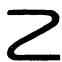
\includegraphics[keepaspectratio]{images/part002_3e739bde.jpg}}

We can show that the strong dual of a metrizable Montel space \(E\) is not metrizable if \(E\) is infinite dimensional (IV, p.~57, exerc. 1).

\section{DUAL OF A FRÉCHET SPACE}

\subsection{Semi-barrelled spaces}

PROPOSITION 1. --- Let E be a locally convex space. The following conditions are equivalent :

\begin{enumerate}
\def\labelenumi{(\roman{enumi})}
\item
  Let U be a subset of E which absorbs every bounded subset of E, and which is the intersection of a sequence of convex, balanced and closed neighbourhoods of 0 in E. Then U is a neighbourhood of 0 in E.
\item
  For every locally convex space \(\mathbf{F}\) , every bounded subset of \(\mathcal{L}_{\mathfrak{b}}(\mathbf{E};\mathbf{F})\) which is the union of a countable family of equicontinuous subsets, is equicontinuous.
\item
  In the strong dual \(E_{b}^{\prime}\) of E, every bounded subset which is the union of a countable family of equicontinuous subsets, is equicontinuous.
\end{enumerate}

It is clear that (iii) is a particular case of (ii).

\begin{enumerate}
\def\labelenumi{(\roman{enumi})}
\item
  \(\Rightarrow\) (ii): let H be a bounded subset of \(\mathcal{L}_b(E;F)\) , and let \((\mathrm{H}_n)\) be a sequence of equicontinuous subsets of \(\mathcal{L}_b(E;F)\) such that \(\mathrm{H} = \bigcup_{n}\mathrm{H}_{n}\) . Let V be a convex, balanced and closed neighbourhood of 0 in F. For every \(n\) , the set \(\mathrm{W}_n = \bigcap_{u\in \mathrm{H}_n}u^{-1}(\mathrm{V})\) is a convex, balanced and closed neighbourhood of 0 in E since \(\mathrm{H}_n\) is equicontinuous. The set \(\mathrm{W} = \bigcap_{u\in \mathrm{H}}u^{-1}(\mathrm{V})\) absorbs every bounded subset of E, since H is bounded in \(\mathcal{L}_b(E;F)\) (III, p.~22), and we have \(\mathrm{W} = \bigcap_{n}\mathrm{W}_{n}\) . If E satisfies (i), then the set W is a neighbourhood of 0 in E, hence H is equicontinuous.
\item
  \(\Rightarrow\) (i): let \((\mathrm{U}_n)\) be a sequence of convex, balanced and closed neighbourhoods of 0 in E. We assume that the set \(\mathbf{U} = \bigcap_{n}\mathbf{U}_{n}\) absorbs every bounded subset of E, hence that its polar \(\mathbf{U}^{\circ}\) is bounded in \(\mathbf{E}_b^\prime\) . Then the set \(\mathbf{B} = \bigcup_{n}\mathbf{U}_{n}^{\circ}\) is contained in \(\mathbf{U}^{\circ}\) , hence is bounded in \(\mathbf{E}_b^\prime\) . If E satisfies (iii), the set B is equicontinuous in \(\mathbf{E}'\) ; consequently, the polar \(\mathbf{B}^{\circ} = \bigcap_{n}(\mathbf{U}_{n}^{\circ})^{\circ} = \bigcap_{n}\mathbf{U}_{n} = \mathbf{U}\) of B in E is a neighbourhood of 0 in E.
\end{enumerate}

DEFINITION 1. --- A locally convex space E is said to be semi-barrelled if it satisfies the equivalent conditions of prop. 1.

Every barrelled space is semi-barrelled. This is also true for every bornological space (III, p.~22, prop. 10).

\subsection{Dual of a locally convex metrizable space}

PROPOSITION 2. --- Let E be a locally convex metrizable space and F its strong dual. The space F is complete, semi-barrelled and satisfies the following condition :

(DB) There exists a sequence \((\mathbf{A}_n)_{n\in \mathbb{N}}\) of bounded subsets of \(\mathbf{F}\) such that every bounded subset of \(\mathbf{F}\) is contained in one of the \(\mathbf{A}_n\) .

The space E is bornological (III, p.~12, prop. 2), hence its strong dual is complete (III, p.~23, cor. 1).

Let \((\mathrm{V}_{n})_{n\in\mathbf{N}}\) be a decreasing sequence of neighbourhoods of 0 in E, such that every neighbourhood of 0 in E contains one of the \(V_{n}\) . Let \(A_{n}\) be the polar of \(V_{n}\) in F. Since E is bornological, every bounded subset of F is equicontinuous (III, p.~22, prop. 10), therefore contained in one of the \(A_{n}\) . In other words, the space F satisfies the condition (DB).

We now show that F is semi-barrelled. Let \((\mathrm{U}_{n})_{n\in\mathbf{N}}\) be a sequence of convex, balanced and closed neighbourhoods of 0 in F. We assume that the set \(U=\bigcap_{n}U_{n}\) absorbs every bounded subset of F. We shall prove that U is a neighbourhood of 0 in F. For this, we shall construct, by induction on the integer \(n\geqslant0\) , real numbers \(\lambda_{n}>0\) and convex balanced neighbourhoods \(W_{n}\) of 0 in F, whose which are closed for \(\sigma(\mathrm{F},\mathrm{E})\) , and satisfy the following relations

\[
\lambda_ {n} \mathrm{A} _ {n} \subset \frac {1}{2} \mathrm{U} \cap \left(\bigcap_ {0 \leqslant i <   n} \mathrm{W} _ {i}\right)\tag{1}
\]

\[
\bigcup_ {0 \leqslant i \leqslant n} \lambda_ {i} \mathrm{A} _ {i} \subset \mathrm{W} _ {n} \subset \mathrm{U} _ {n}.\tag{2}
\]

Suppose that the numbers \(\lambda_{i}\) and the sets \(\mathrm{W}_i\) have been constructed for \(0 \leqslant i < n\) . By the hypothesis, the set U absorbs the bounded subsets of F; moreover, for \(0 \leqslant i < n\) , \(\mathrm{W}_i\) is a neighbourhood of 0 in F, hence absorbs the bounded subsets of F. We can therefore find a number \(\lambda_{n} > 0\) satisfying (1). Let C denote the closed convex balanced envelope, for \(\sigma(\mathrm{F}, \mathrm{E})\) , of \(\bigcup_{0 \leqslant i \leqslant n} \lambda_i \mathrm{A}_i\) ; the set C is equicontinuous,

hence compact for \(\sigma(\mathrm{F},\mathrm{E})\) (III, p.~17, cor. 2). Since \(\mathrm{U}_n\) is a neighbourhood of 0 in F, there exists a bounded subset B of E such that \(\mathbf{B}^{\circ}\subset\frac{1}{2}\mathbf{U}_{n}\) . Put \(\mathrm{W}_n=\mathrm{C}+\mathrm{B}^{\circ}\) . Since \(\mathbf{B}^{\circ}\) is a neighbourhood of 0 in F, we see that \(\mathrm{W}_n\) is a convex and balanced neighbourhood of 0 in F. In addition, C is compact and \(\mathbf{B}^{\circ}\) closed for \(\sigma(\mathrm{F},\mathrm{E})\) ; by cor. 1 of GT, III, § 4, No.~1, \(\mathrm{W}_n\) is closed for \(\sigma(\mathrm{F},\mathrm{E})\) . Finally, we have \(\mathbf{C}\subset\frac{1}{2}\mathbf{U}\subset\frac{1}{2}\mathbf{U}_n\) and \(\mathbf{B}^{\circ}\subset\frac{1}{2}\mathbf{U}_n\) , hence \(\mathrm{W}_n\subset\mathrm{U}_n\) since \(\mathrm{U}_n\) is convex. We have thus established (2).

Put
\[
\mathrm{W} = \bigcap_ {n} \mathrm{W} _ {n}
\]

then
\[
\mathbf {W} \subset \mathbf {U}
\]

By (1) and (2), we have
\[
\lambda_ {i} \mathrm{A} _ {i} \subset \mathrm{W} _ {j} \quad \text {for all } i \text { and } j
\]

in N, and so \(\lambda_{i}A_{i}\subset W\) for all \(i\in N\) . In particular, W is absorbent, hence is a barrel for \(\sigma(\mathrm{F},\mathrm{E})\) . By remark 3 of IV, p.~4, W is a neighbourhood of 0 in F. A fortiori, U is a neighbourhood of 0 in F, and F is semi-barrelled.

The following corollary extends the Banach-Steinhaus theorem to the dual of a Fréchet space (cf.~III, p.~25, cor. 2).

COROLLARY. --- Let G be a Hausdorff locally convex space, and let \((u_{n})\) be a sequence of linear mappings from F into G, converging simply to a mapping u from F into G. Then u is continuous, and the sequence \((u_{n})\) converges to u uniformly on every pre-compact subset of F.

Since F is complete, the set of all \(u_{n}\) , which is bounded for the topology of simple convergence, is bounded in \(\mathcal{L}_{b}(F;G)\) (III, p.~27, cor. 1). Since the space F is semibarrelled (prop. 2), every countable and bounded subset of \(\mathcal{L}_{b}(F;G)\) is equicontinuous by prop. 1 of IV, p.~21. Therefore the set of the \(u_{n}\) is equicontinuous, and the corollary follows from III, p.~18, corollary.

\subsection{Bidual of a locally convex metrizable space}

PROPOSITION 3. --- Let E be a locally convex metrizable space, \(E_{b}^{\prime}\) its strong dual and G a Fréchet space. The space \(\mathcal{L}_{b}(E_{b}^{\prime}; G)\) is a Fréchet space.

By prop. 2 (IV, p.~22), there exists a sequence \((\mathrm{A}_n)\) of bounded subsets of \(\mathrm{E}_b'\) such that every bounded subset of \(\mathrm{E}_b'\) is contained in one of the \(\mathrm{A}_n\) . Let \((\mathrm{V}_n)\) be a countable fundamental system of neighbourhoods of 0 in \(\mathbf{G}\) . Let \(\mathrm{H}_{mn}\) be the set of linear mappings \(u\) from \(\mathrm{E}_b'\) into \(\mathbf{G}\) such that \(u(\mathrm{A}_m) \subset \mathrm{V}_n\) . Then \((\mathrm{H}_{mn})\) is a fundamental system of neighbourhoods of 0 in \(\mathcal{L}_b(\mathrm{E}_b'; \mathrm{G})\) , and the latter space is then metrizable.

To show that \(\mathcal{L}_b(\mathrm{E}_b';\mathbf{G})\) is complete, it is enough to prove that every Cauchy sequence \((u_n)\) in this space is convergent; since \(\mathbf{G}\) is complete, there exists a linear mapping \(u:\mathrm{E}_b' \to \mathbf{G}\) such that \((u_n)\) converges simply to \(u\) . By IV, p.~23, corollary, we have \(u \in \mathcal{L}_h(\mathrm{E}_h';\mathbf{G})\) . It then follows from prop. 5 of GT, X, § 1, No.~5, that \((u_n)\) converges to \(u\) in \(\mathcal{L}_b(\mathrm{E}_b';\mathbf{G})\) .

COROLLARY. --- The bidual of a locally convex metrizable space is a Fréchet space.

\subsection{Dual of a reflexive Fréchet space}

PROPOSITION 4. --- Let E be a reflexive Fréchet space. The strong dual \(E_{b}^{\prime}\) of E is the inductive limit of a sequence of Banach spaces.

Let \((\mathrm{V}_{n})_{n\in\mathbf{N}}\) be a decreasing sequence of convex, balanced and closed neighbourhoods of 0 in E, such that every neighbourhood of 0 in E contains one of the \(V_{n}\) . Let \(A_{n}\) be the polar of \(V_{n}\) in \(E'\) . Then \(A_{n}\) is convex, balanced and compact for \(\sigma(\mathrm{E}',\mathrm{E})\) ; by III, p.~8, corollary the space \(E_{A_{n}}'\) is a Banach space. We shall prove that \(E_{b}'\) is the inductive limit of the spaces \(E_{A_{n}}'\) ; in other words, that every convex and balanced subset U of \(E'\) which absorbs each of the \(A_{n}\) is a neighbourhood of 0 in \(E_{b}'\) . For every \(n\in\mathbf{N}\) , choose a real number \(\lambda_{n}>0\) such that \(\lambda_{n}A_{n}\subset U\) . Let \(B_{n}\) be the convex envelope of the set \(\bigcup_{0\leqslant i\leqslant n}\lambda_{i}A_{i}\) ; put \(V=\bigcup_{n}B_{n}\) , then \(V\subset U\) . For every \(n\in\mathbf{N}\) , the set \(B_{n}\) is convex, balanced and compact for \(\sigma(\mathrm{E}',\mathrm{E})\) (II, p.~14, prop. 15).

Now we shall show that \(\frac{1}{2}\mathrm{V}^{\circ \circ}\subset \mathrm{V}\) . Let \(x\in \mathrm{E}_b^\prime -\mathrm{V}\) ; for every \(n\in \mathbf{N}\) , we have \(x\notin \mathbf{B}_n\) , and since \(\mathbf{B}_n\) is closed for \(\sigma (\mathrm{E}',\mathrm{E})\) there exists an element \(y_{n}\) in \(\mathbf{B}_n^\circ\) such that \(\langle y_n, x \rangle = 1\) (II, p.~38, prop. 4). Since E is reflexive, every bounded subset of E is relatively compact for \(\sigma(E, E')\) (IV, p.~16, th. 2). By the definition of \(B_n\) , we have

\[
\lambda_ {i} y _ {n} \in \mathrm{V} _ {i} \quad \text { for   all } \quad n \geqslant i  ,\tag{3}
\]

hence the sequence \((y_{n})\) is bounded. Let \(y\) be a limit point of \((y_{n})\) for the topology \(\sigma(\mathrm{E},\mathrm{E}')\) . We have \(y\in\mathrm{V}^{\circ}=\bigcap_{n}\mathrm{B}_{n}^{\circ}\) and \(\langle y,x\rangle=1\) . Hence \(x\notin\frac{1}{2}\mathrm{V}^{\circ\circ}\) , and so we have the inclusion \(\frac{1}{2}\mathrm{V}^{\circ\circ}\subset\mathrm{V}\) and a fortiori, \(\frac{1}{2}\mathrm{V}^{\circ\circ}\subset\mathrm{U}\) .

Since every bounded subset of \(E_{b}^{\prime}\) is contained in one of the sets \(A_{n}\) , the set \(V = \bigcup_{n} B_{n}\)

absorbs every bounded subset of \(E_{b}^{\prime}\) . Consequently, \(V^{\circ}\) is bounded in E, hence \(\frac{1}{2}V^{\circ\circ}\) is a neighbourhood of 0 in \(E_{b}^{\prime}\) . A fortiori, U is a neighbourhood of 0 in \(E_{b}^{\prime}\) .

COROLLARY. --- The strong dual of a reflexive Fréchet space is bornological and barrelled.

An inductive limit of Banach spaces is bornological by definition. Further, a Banach space is barrelled (III, p.~25, corollary) and every inductive limit of barrelled spaces is a barrelled space (III, p.~25, cor. 3).

\subsection{The topology of compact convergence on the dual of a Fréchet space}

THEOREM 1 (Banach-Dieudonné). --- Let E be a locally convex metrizable space. The following topologies coincide on the dual E' of E :

\begin{enumerate}
\def\labelenumi{\alph{enumi})}
\item
  the topology \(\mathcal{T}_{\mathfrak{N}}\) of \(\mathfrak{N}\) -convergence, where \(\mathfrak{N}\) is the family of subsets of \(E\) each consisting of points of a sequence converging to 0;
\item
  the topology \(\mathcal{T}_{\mathrm{c}}\) of uniform convergence on compact subsets of E;
\item
  the topology \(\mathcal{T}_{pc}\) of uniform convergence on precompact subsets of E;
\item
  the topology \(\mathcal{T}_f\) which is the finest topology inducing the same topology as \(\sigma(\mathrm{E}',\mathrm{E})\) on every equicontinuous subset of \(\mathrm{E}'\) .
\end{enumerate}

First observe that a subset A of \(E'\) is closed for \(T_{f}\) if and only if \(A \cap H\) is closed for \(\sigma(E', E)\) for every subset H of \(E'\) which is equicontinuous and closed for \(\sigma(E', E)\) . The weak topology \(\sigma(E', E)\) and \(T_{pc}\) induce the same topology on every equicontinuous subset of \(E'\) (III, p.~17, prop. 5). Consequently each of the topologies \(T_{R}\) , \(T_{c}\) , \(T_{pc}\) , \(T_{f}\) is coarser than the one following it. It is therefore enough to prove that \(T_{R}\) is finer than \(T_{f}\) . Moreover, every translation in \(E'\) is a homeomorphism for \(T_{f}\) . Hence it is enough to prove that, if F is a subset of \(E'\) which is closed for \(T_{f}\) , and does not contain 0, then there exists a set \(S \in R\) such that \(S^{\circ} \cap F = \varnothing\) .

Let \((\mathbf{U}_{n})_{n\geqslant0}\) be a decreasing sequence of neighbourhoods of 0 in E forming a fundamental system of neighbourhoods of 0. We shall construct, by induction on \(n\geqslant0\) , finite sets \(X_{n}\) such that we have

\[
\mathrm{X} _ {n} \subset \mathrm{U} _ {n}\tag{4}
\]

\[
\left(\bigcup_ {0 \leqslant p \leqslant n} \mathrm{X} _ {p}\right) ^ {\circ} \cap \mathrm{U} _ {n + 1} ^ {\circ} \cap \mathrm{F} = \varnothing\tag{5}
\]

for every integer \(n \geqslant 0\) . Let \(m \geqslant 0\) be an integer such that \(X_{n}\) has been constructed for \(0 \leqslant n < m\) and satisfies (4) and (5) for \(0 \leqslant n < m\) . For every \(x \in U_{m}\) , put

\[
\mathrm{F} _ {x} = \big (\bigcup_ {0 \leqslant p <   m} \mathrm{X} _ {p} \big) ^ {\circ} \cap \{x \} ^ {\circ} \cap \mathrm{U} _ {m + 1} ^ {\circ} \cap \mathrm{F}.
\]

Formula (5) with \(n = m - 1\) implies that \(\bigcap_{x\in \mathrm{U}_m}\mathrm{F}_x = \emptyset\) . Further, the set \(\mathrm{U}_{m + 1}^{\circ}\) is equicontinuous, and compact for \(\sigma (\mathrm{E}',\mathrm{E})\) . In view of the definition of \(\mathcal{T}_f\) , each of the sets \(\mathrm{F}_x\) is compact for \(\sigma (\mathrm{E}',\mathrm{E})\) ; therefore there exists a finite subset \(\mathrm{X}_m\) of \(\mathrm{U}_m\) such that \(\bigcap_{x\in \mathrm{U}_m}\mathrm{F}_x = \emptyset\) , i.e.~relation (5) is satisfied for \(n = m\) .

Put \(S = \bigcup_{n\geqslant 0}X_n\) . We have \(X_{n}\subset U_{p}\) for \(n\geqslant p\) , therefore \(S\) is the set of points of a sequence which converges to 0 in \(E\) . From (5) we deduce that \(S^{\circ}\cap U_{n + 1}^{\circ}\cap F = \emptyset\) , and since \(E'\) is the union of the sequence of sets \(U_{n + 1}^{\circ}\) , we get \(S^{\circ}\cap F = \emptyset\) .

COROLLARY 1. --- Let E be a locally convex metrizable space. Every precompact subset of E is contained in the closed convex balanced envelope of the set of points of a sequence converging to 0.

This follows from the fact that the topologies \(\mathcal{T}_{pc}\) and \(\mathcal{T}_{\mathfrak{N}}\) are identical, on account of prop. 2 of III, p.~15.

COROLLARY 2. --- Let E be a Fréchet space. In order that a convex subset A of the dual E' of E be closed for \(\sigma(E', E)\) , it is necessary and sufficient that \(A \cap U^{\circ}\) is closed for \(\sigma(E', E)\) for every neighbourhood U of 0 in E.

Since E is complete, the topology \(T_{c}\) on \(E'\) is compatible with the duality between \(E'\) and E (IV, p.~3, Example); consequently the closed convex subsets in \(E'\) are the same for \(T_{c}\) and \(\sigma(E', E)\) (IV, p.~1, prop. 1). The corollary then follows from the identity of the topologies \(T_{c}\) and \(T_{f}\) .

Recall (I, p.~13) that the hyperplanes of E' which are closed for \(\sigma(\mathrm{E}', \mathrm{E})\) are the kernels of linear forms on E' associated with elements of E. Cor. 2 therefore gives another proof (for Fréchet spaces) of cor. 1 of III, p.~21.

COROLLARY 3. --- Let E be a Banach space and M a vector subspace of the dual E' of E. In order that M be closed for the weak topology \(\sigma(E', E)\) , it is necessary and sufficient that its intersection with the unit ball (closed) in E' be closed for \(\sigma(E', E)\) .

Example. --- * Let H be a hilbertian space satisfying the first axiom of countability; let \(H_{\sigma}\) denote the space H with the weakened topology assigned to it. Let \(\mathcal{L}^{1}(H)\) be the Banach space of nuclear endomorphisms of H (V, p.~51, and TS, V); the norm in \(\mathcal{L}^{1}(H)\) is defined by \(\|u\|_{1} = \operatorname{Tr}((u^{*}u)^{1/2})\) . We can identify \(\mathcal{L}(H)\) with the dual of the Banach space \(\mathcal{L}^{1}(H)\) by associating the linear form \(\phi_{u}: v \mapsto \operatorname{Tr}(uv)\) on \(\mathcal{L}^{1}(H)\) with every \(u \in \mathcal{L}(H)\) . Let A be a sub-algebra of \(\mathcal{L}(H)\) , containing 1 and stable under \(u \mapsto u^{*}\) ; this is a von Neumann algebra if and only if it is closed in \(\mathcal{L}(H)\) for the weak topology \(\sigma(\mathcal{L}(H), \mathcal{L}^{1}(H))\) . From cor. 3, we deduce the following criterion: for A to be a von Neumann algebra, it is necessary and sufficient that if \((u_{n})\) is any sequence of elements of A with norm \(\leqslant 1\) having a limit u in the space \(\mathcal{L}_{s}(H; H_{\sigma})\) , then u belongs to A.

\subsection{Separately continuous bilinear mappings}

Lemma 1. --- Let E and F be two locally convex metrizable spaces, and u be a continuous linear mapping from \(E_{b}^{\prime}\) into F. Then there exists a neighbourhood U of 0 in \(E_{b}^{\prime}\) whose image under u is bounded in F.

Let \((\mathrm{U}_n)_{n\in \mathbf{N}}\) (resp. \((\mathrm{V}_n)_{n\in \mathbf{N}}\) ) be a fundamental system of neighbourhoods of 0 in E (resp. F). We assume that the sets \(\mathrm{U}_n\) are balanced and form a decreasing sequence. Since \(u\) is continuous, for every \(n\in \mathbf{N}\) , there exists a bounded set \(\mathrm{B}_n\) in E such that \(u(\mathrm{B}_n^\circ)\subset \mathrm{V}_n\) . Since \(\mathrm{B}_n\) is bounded, there exists a real number \(\lambda_n > 0\) such that \(\lambda_{n}\mathrm{B}_{n}\subset \mathrm{U}_{n}\) . Put \(\mathrm{B} = \bigcup_{n\in \mathbf{N}}\lambda_n\mathrm{B}_n\) .

We shall prove that the set B is bounded in E, in other words that for every integer \(m \geqslant 0\) , there exists a real number \(\mu > 0\) such that \(\mu B \subset U_{m}\) . Since the sets \(B_{n}\) are bounded, there exists a real number \(\mu\) such that \(0 < \mu \leqslant 1\) and such that \(\mu \cdot (\lambda_{n} B_{n}) \subset U_{m}\) for \(0 \leqslant n \leqslant m\) ; we have also \(\lambda_{n} B_{n} \subset U_{n} \subset U_{m}\) if n \textgreater{} m; hence \(\mu B \subset U_{m}\) since \(U_{m}\) is balanced.

Let \(\mathbf{U}\) be the polar of \(\mathbf{B}\) in \(\mathrm{E}_b'\) . This is a neighbourhood of 0 in \(\mathrm{E}_b'\) and we have \(\lambda_n\mathrm{B}^\circ \subset \mathrm{B}_n^\circ\) , hence \(\lambda_n u(\mathrm{U}) \subset \mathrm{V}_n\) for all \(n \in \mathbf{N}\) . Consequently \(u(\mathrm{U})\) is bounded in \(\mathrm{F}\) .

THEOREM 2. --- Let \(E_{1}\) and \(E_{2}\) be two reflexive Fréchet spaces, and G a locally convex Hausdorff space. For i = 1, 2, let \(F_{i}\) be the strong dual of \(E_{i}\) . Then every separately continuous bilinear mapping \(u: F_{1} \times F_{2} \to G\) is continuous.

The space G is isomorphic to a subspace of a product of Banach spaces (II, p.~5, prop. 3). Therefore it is enough to prove the theorem under the additional hypothesis that G is a Banach space. But \(F_{1}\) is barrelled and \(F_{2}\) bornological (IV, p.~24, corollary), and \(\mathcal{L}_{b}(F_{2}; G)\) is a Fréchet space (IV, p.~23, prop. 3). Let v denote the linear mapping from \(F_{1}\) into \(\mathcal{L}_{b}(F_{2}, G)\) associated with u by the relation

\[
u (x _ {1}, x _ {2}) = v (x _ {1}) \left(x _ {2}\right) \quad \left(x _ {1} \in \mathrm{F} _ {1}, x _ {2} \in \mathrm{F} _ {2}\right).
\]

Since \(F_{1}\) is barrelled and u separately continuous, v is continuous (III, p.~31, prop. 6). Since v is continuous, lemma 1 implies the existence of a neighbourhood \(U_{1}\) of 0 in \(F_{1}\) whose image under v is bounded in \(\mathcal{L}_{b}(F_{2}; G)\) . In other words, for every bounded subset \(B_{2}\) in \(F_{2}\) , the set \(u(U_{1} \times B_{2})\) is bounded in the Banach space G. Let \(U_{2}\) be the set of all \(x_{2} \in F_{2}\) such that \(\|u(x_{1}, x_{2})\| \leqslant 1\) for all \(x_{1} \in U_{1}\) . The set \(U_{2}\) then absorbs every bounded subset; since \(F_{2}\) is bornological, \(U_{2}\) is a neighbourhood of 0 in \(F_{2}\) , and this proves that u is continuous.

\section{STRICT MORPHISMS OF FRÉCHET SPACES}

For every locally convex space E, let S(E) denote the set of all continuous seminorms on E. For every \(p \in \mathrm{S}(\mathrm{E})\) , let \(H_{p}\) denote the set of all linear forms f on E such that \(|f| \leqslant p\) . The family \((\mathrm{H}_{p})_{p \in \mathrm{S}(\mathrm{E})}\) is a base for the bornology consisting of equicontinuous subsets of \(E'\) .

\subsection{Characterizations of strict morphisms}

PROPOSITION 1. --- Let E and F be two locally convex spaces and u a continuous linear mapping from E into F. In order that u be a strict morphism, it is necessary and sufficient that the following condition be satisfied :

(MS) For every semi-norm \(p \in \mathrm{S}(\mathrm{E})\) , which is null on the kernel of \(u\) , there exists \(q\) in \(\mathrm{S}(\mathrm{F})\) such that \(p \leqslant q \circ u\) .

Let N be the kernel and M the image of u; we introduce the canonical decomposition of u, let

\[
\mathrm{E} \xrightarrow {\pi} \mathrm{E} / \mathrm{N} \xrightarrow {\tilde {u}} \mathrm{M} \xrightarrow {\iota} \mathrm{F}.
\]

The continuous semi-norms on E which are null on N, are the semi-norms \(p_{1} \circ \pi\) where \(p_{1}\) ranges over S(E/N); similarly S(M) consists of the semi-norms \(q_{1}\) for which there exists \(q \in \mathrm{S}(F)\) with \(q_{1} \leqslant q/F\) . Finally, u is a strict morphism if and only if the bijective continuous linear mapping \(\tilde{u}\) has a continuous inverse; this also means that every semi-norm in S(E/N) is of the form \(q_{1} \circ \tilde{u}\) with \(q_{1}\) in S(M). Prop. 1 follows immediately from these remarks.

PROPOSITION 2. --- Let E and F be two Hausdorff locally convex spaces and u a continuous linear mapping from E into F. In order that u be a strict morphism, it is necessary and sufficient that its transpose \({}^t u\): F' → E' satisfy the following conditions :

\begin{enumerate}
\def\labelenumi{\alph{enumi})}
\item
  The image of \(^{t}u\) is closed in \(E'\) for \(\sigma(E', E)\) .
\item
  Every equicontinuous subset of \(\mathbf{E}'\) , contained in the image of \({}^t u\) is the image under \({}^t u\) of an equicontinuous subset of \(\mathbf{F}'\) .
\end{enumerate}

If this is so, we have \(\operatorname{Ker}^t u = (\operatorname{Im} u)^\circ\) and \(\operatorname{Im}^t u = (\operatorname{Ker} u)^\circ\) and there exist canonical isomorphisms from \(\operatorname{Coker}^t u\) onto the dual of \(\operatorname{Ker} u\) and from \(\operatorname{Ker}^t u\) onto the dual of \(\operatorname{Coker} u\) .

Let N be the kernel and I the image of u. By cor. 2 of II, p.~47, the kernel of \(^{t}u\) is the orthogonal of I, and the closure of the image of \(^{t}u\) for \(\sigma(E', E)\) is the orthogonal \(N^{\circ}\) of N. The conjunction of a) and b) is then equivalent to the following condition:

b') Every equicontinuous subset of \(E'\) contained in \(N^{\circ}\) is the image under \(^{t}u\) of an equicontinuous subset of \(F'\) .

Since \(N^{\circ}\) can be identified with the dual of E/N, prop. 9, (i) of IV, p.~8, shows that the equicontinuous subsets of \(E'\) contained in \(N^{\circ}\) are the sets which are contained in a set of the form \(H_{p}\) , where p is a continuous semi-norm on E, vanishing on N. The condition \(b')\) then says that, for every semi-norm \(p \in \mathrm{S}(\mathrm{E})\) which is null on N, there exists \(q \in \mathrm{S}(\mathrm{F})\) such that \(\mathrm{H}_{p} \subset {}^{t}u(\mathrm{H}_{q})\) . By Hahn-Banach theorem (II, p.~23, cor. 1 and 2, p.~63, th. 1 and cor. 1), we have \(u(\mathrm{H}_{q}) = \mathrm{H}_{q \circ u}\) , and the relations \(H_{p} \subset H_{p'}\) and \(p \leqslant p'\) are equivalent for all semi-norms p and \(p'\) in S(E). Consequently, the relation \(H_{p} \subset {}^{t}u(\mathrm{H}_{q})\) is equivalent to the relation \(p \leqslant q \circ u\) . By prop. 1, property \(b')\) implies that u is a strict morphism.

Suppose that \(u\) is a strict morphism. We have already seen that the kernel of \(^t u\) is the orthogonal of I and the image of \(^t u\) is the orthogonal of N. The cokernel of u is the space F/I and its dual can be identified with \(I^{\circ} = Ker^{t}u\) . Similarly, the dual of N = Ker u can be identified with \(E^{\prime}/N^{\circ}\) (IV, p.~8), i.e.~with the cokernel of \(^{t}u\) since \(N^{\circ}\) is the image of \(^{t}u\) .

Remark. --- With the notations of prop. 2, property \(b'\) ) also implies that \(u\) is a strict morphism for the weakened topologies (II, p.~49, cor. 3).

PROPOSITION 3. --- Let E and F be two locally convex spaces, and u a continuous linear mapping from E into F. We assume that E is Hausdorff and that F is metrizable. For u to be a strict morphism, it is necessary and sufficient that the image of \({}^t u\) be closed in E' for the weak topology \(\sigma(E', E)\) .

The necessity follows from prop. 2.

Conversely, suppose that the image of \(^t u\) is closed for \(\sigma(E', E)\) and introduce the canonical decomposition of \(u\) as in the proof of prop. 1. By the above remarks, the inverse mapping \(\tilde{u}^{-1}\) of \(\tilde{u}\) is continuous for the weakened topologies. But the subspace \(M = u(E)\) of F is metrizable, hence bornological (III, p.~12, prop. 2); consequently (IV, p.~7, prop. 7, (ii)), \(\tilde{u}^{-1}\) is continuous, hence \(u\) is a strict morphism.
